
\documentclass[font=arial,acronym,symbols]{fei}

\usepackage[utf8]{inputenc}
\usepackage{graphicx}
\usepackage{float}

%%%% -- Configuracoes Iniciais
%%%%%%%%%%%%%%%%%%%%%%%%%%%%%%%%%%%%%%%%%%%%%%%%%%%%%%%%%%%%%%%%%%%%%%%%%%%%%%%%%%%%%%%%%%%%%%%%%%%%%%%%%

\author{Adalberto Nassu Pompolo}
%\cidade{Cidade}
%\instituicao{Instituição de Ensino}
\title{Utilização de uma rede \textit{Multilayer Perceptron} para busca semântica de código-fonte a partir de linguagem natural}

% comando para inserção de subfloats do tipo figure, usado aqui no template
% remova este comando se for usar o pacote subfig
% não recomendo o pacote subcaption
% \newsubfloat{figure}

% \subtitulo{subtítulo}

%%%%%%%%%%%%%%%%%%%%%%%%%%%%%%%%%%%%%%%%%%%%%%%%%%%%%%%%%%%%%%%%%%%%%%%%%%%%%%%%%%%%%%%%%%%%%%%%%%%%%%%%%
%%%% -- Entradas Listas de Abreviaturas e Simbolos
%%%%%%%%%%%%%%%%%%%%%%%%%%%%%%%%%%%%%%%%%%%%%%%%%%%%%%%%%%%%%%%%%%%%%%%%%%%%%%%%%%%%%%%%%%%%%%%%%%%%%%%%%
%% -- Abreviaturas
% Intro
\newacronym{fei}{FEI}{Centro Universitário da FEI}
\newacronym{nlp}{NLP}{\textit{Natural Language Processing}}
\newacronym{mlp}{MLP}{\textit{Multilayer perceptron}}
% Related works
\newacronym{mrr}{MRR}{\textit{Mean Reciprocal Rank}}
\newacronym{deepcs}{DeepCS}{\textit{Deep Code Search}}
\newacronym{nbow}{NBOW}{\textit{Neural bag-of-words}}
\newacronym{ndcg}{NDCG}{\textit{Normalized Discounted Cumulative Gain}}
\newacronym{unif}{UNIF}{\textit{Embedding Unification}}
\newacronym{ncs}{NCS}{\textit{Neural Code Search}}
\newacronym{mman}{MMAN}{\textit{Multi-Modal Attention Network}}
\newacronym{lstm}{LSTM}{\textit{Long short-term memory}}
\newacronym{ggnn}{GGNN}{\textit{Gated Graph Neural Network}}
\newacronym{coacor}{CoaCor}{\textit{Code annotation for Code retrieval}}
\newacronym{bleu}{BLEU}{\textit{BiLingual Evaluation Understudy}}
\newacronym{graphcodebert}{GraphCodeBERT}{GraphCodeBERT}
\newacronym{ast}{AST}{\textit{Abstract Syntax Tree}}
\newacronym{birnn}{BiRNN}{\textit{Bidirectional Recurrent Neural Network}}
\newacronym{tabcs}{TabCS}{\textit{Twostage Attention-Based model for Code Search}}
\newacronym{carlcscnn}{CARLCS-CNN}{\textit{Co-Attentive Representation Learning Code Search-CNN}}
\newacronym[longplural={Campos aleatórios de Markov}]{cam}{CAM}{Campo aleatório de Markov}
\newacronym{ir}{IR}{\textit{Information Retrieval}}
\newacronym{dl}{DL}{\textit{Deep Learning}}
\newacronym{bert}{BERT}{\textit{Bidirectional Encoder Representations from Transformers}}
\newacronym[longplural=\textit{Application Programming Interfaces}]{api}{API}{\textit{Application Programming Interface}}
\newacronym{cqil}{CQIL}{\textit{CodeQuery Interaction Learner}}
\newacronym{co3}{CO3}{CO3}
\newacronym{sql}{SQL}{\textit{Structured Query Language}}
\newacronym{adacs}{AdaCS}{\textit{Adaptive Deep Code Search}}
\newacronym{tbcnn}{TBCNN}{\textit{Tree-based CNN}}
\newacronym{bilstm}{Bi-LSTM}{\textit{Bidirectional Long Short-Term Memory}}
\newacronym{cradle}{CRaDLe}{\textit{Code Retrieval based on statement-level semantic Dependency Learning}}
\newacronym{gnn}{GNN}{\textit{Graph Neural Networks}}
\newacronym{degraphcs}{DeGraphCS}{\textit{Deep Graph for Code Search}}
\newacronym{dgms}{DGMS}{\textit{Deep Graph Matching and Searching}}
\newacronym{cdcs}{CDCS}{\textit{Cross-Domain Deep Code Search}}
\newacronym{quecos}{QueCos}{\textit{Query-enriched Code search model}}
\newacronym{coshc}{CoSHC}{\textit{Accelerating Semantic Code Search with Deep Hashing and Code Classification}}
\newacronym{rnn}{RNN}{Rede Neural Recorrente}
\newacronym{csrs}{CSRS}{\textit{Code Search with Relevance Matching and Semantic Matching}}
\newacronym{bpe}{BPE}{\textit{Byte-Pair Encoding}}
\newacronym{gpt2}{GPT2}{\textit{Generative Pretrained Transformer 2}}
\newacronym{roberta}{RoBERTa}{RoBERTa}
\newacronym[longplural=\textit{Reciprocal Ranks}]{rr}{RR}{\textit{Reciprocal Rank}}
\newacronym{distilroberta}{DistilRoBERTa}{DistilRoBERTa}
\newacronym{relu}{ReLU}{\textit{Rectified Linear Unit}}

%% -- Simbolos
% \newglossaryentry{A}{type=symbols,name={\ensuremath{A}},sort=a,description={exchanger total heat transfer area, $m^2$}}
% \newglossaryentry{G}{type=symbols,name={\ensuremath{G}},sort=g,description={exchanger flow-stream mass velocity, $kg/(s m^2)$}}
% \newglossaryentry{f}{type=symbols,name={\ensuremath{j}},sort=j,description={friction factor, dimensionless}}
% \newglossaryentry{deltap}{type=symbols,name={\ensuremath{\Delta P}},sort=p,description={pressure drop, $Pa$}}
% \newglossaryentry{nu}{type=symbols,name={\ensuremath{\nu}},sort=b,description={specific volume, $m^3/kg$}}
% \newglossaryentry{beta}{type=symbols,name={\ensuremath{\beta}},sort=b,description={ratio of free-flow area $A_{ff}$ and frontal area $A_{fr}$ of one side of exchanger, dimensionless}}
% \newglossaryentry{fr}{type=symbols,name={\ensuremath{fr}},sort=fr,description={frontal}}
% \newglossaryentry{in}{type=symbols,name={\ensuremath{i}},sort=in,description={inlet}}
% \newglossaryentry{out}{type=symbols,name={\ensuremath{o}},sort=out,description={outlet}}
%%%%%%%%%%%%%%%%%%%%%%%%%%%%%%%%%%%%%%%%%%%%%%%%%%%%%%%%%%%%%%%%%%%%%%%%%%%%%%%%%%%%%%%%%%%%%%%%%%%%%%%%%

\addbibresource{artigos.bib}

\makeindex

\makeglossaries

\begin{document}

\maketitle

\begin{folhaderosto}
Dissertação de Mestrado, apresentada ao Centro Universitário da FEI para obtenção do título de Mestre em Engenharia Elétrica. Orientado pela Prof. Dr. Leila Cristina Carneiro Bergamasco.
\end{folhaderosto}

\fichacatalografica
\folhadeaprovacao

\dedicatoria{Ao meu avô Adalberto Nassu, e ao meu tio Paulo Henrique Abdalla dos Santos.}
\begin{agradecimentos}
Agradeço a Deus, por ter me sustentado em todos os momentos; aos meus pais, Ciro e Patricia Pompolo - este trabalho também é de vocês; e por fim, ao Centro Universitário FEI e, em especial, aos professores Dra. Leila Bergamasco, Dr. Danilo Perico e Dr. Guilherme Wachs.
\end{agradecimentos}
\begin{epigrafe}
	\epig{Beware of bugs in the above code; I have only proved it correct, not tried it.}{Donald E. Knuth}
	\epig{Something is rotten in the state of Denmark.}{William Shakespeare}
\end{epigrafe}
\begin{resumo}
Ferramentas de busca de código-fonte a partir de linguagem natural são cada vez mais importantes no dia a dia de engenheiros e desenvolvedores de \textit{software}. Atualmente, modelos \textit{transformers} são o estado da arte em diversas tarefas da área de \gls{nlp}, como busca de código-fonte a partir de linguagem natural. Porém, tais modelos requerem muito tempo e recursos computacionais para serem treinados em um determinado domínio (\textit{fine-tuning)}. Por outro lado, redes neurais clássicas, como \gls{mlp} por exemplo, necessitam de menos recursos para seu treinamento, porém não obtém os resultados dos modelos \textit{transformers}. Diante disso, o objetivo do presente trabalho é utilizar uma rede \gls{mlp} para determinar a similaridade entre dois \textit{embeddings}, gerados por redes \textit{transformers}, de dois domínios diferentes: linguagem natural e linguagem de programação. Para tanto, serão utilizados mais de 10000 pares código-fonte/comentário, bem como um conjunto de buscas (\textit{queries}) e seus resultados esperados; ambos oriundos da base de dados \textit{CodeSearchNet} \textcite{Husain2019CodeSearchNetCE}.

\palavraschave{busca de código-fonte. recuperação de código-fonte. linguagem natural. transformers. embedding}
\end{resumo}

\begin{abstract}
Code search tools using natural language queries are becoming an essential tool for software engineers. Nowadays, the transformers models are the state-of-art for several natural language processing tasks such as code search using natural language. However, such models requires a lot of computational resources for training in a specific domain (fine-tuning). On the other hand, classical neural networks such as \gls{mlp} takes less computational resources for training in a specific domain, but it does not achieve the transformers models results. That being said, the goal of this study is to use a \gls{mlp} network to determine the similarity between two transformers embeddings from two different domains: one trained using \gls{nlp} and the other using code snippets. Therefore, it will be used more than 10000 code/comment pairs as well as a annotated queries dataset; both datasets came from the {CodeSearchNet} \textcite{Husain2019CodeSearchNetCE} database.

\keywords{code search. code retrieval. natural language. transformers. embedding.}
\end{abstract}

\glsresetall

% \listoffigures
% \listoftables
% \listofalgorithms
\printglossaries
\tableofcontents

\chapter{Introdução}
\label{chp:introduction}

Busca de código-fonte é uma tarefa essencial no trabalho de engenheiros e desenvolvedores de \textit{software} \cite{Rahman2018EvaluatingHD}. \textcite{Sadowski2015HowDS} mostrou que, em média, um engenheiro realiza 5 sessões de busca de código-fonte com 12 buscas por sessão, totalizando assim 60 buscas por código-fonte durante um dia de trabalho. \textcite{Xia2017WhatDD} também mostra que trechos de código-fonte estão entre os itens mais buscados pelos engenheiros de \textit{software}.

Porém, um dos problemas conhecidos da área de recuperação de informação é o \textit{term mismatch} ou \textit{vocabulary mismatch} \cite{Furnas1987TheVP} \cite{Carpineto2012ASO}. Em busca de código-fonte, esse problema se dá quando os termos da busca providos pelo usuário não coincidem com os termos utilizados nos trechos de código-fonte correspondentes \cite{Nie2016QueryEB}. Além disso, a maioria das ferramentas de busca de código-fonte atuais realizam buscas por correspondência textual. Tais buscas utilizam o termo buscado pelo usuário (tal termo também é chamado de \textit{query}) e procuram códigos-fonte que contenham este mesmo termo. Esse método de busca tende a incorrer no problema de \textit{term mismatch}.

Por exemplo: considere que o engenheiro de \textit{software} queira encontrar códigos-fontes relacionados ao processo de autenticação de um usuário em determinado sistema. Normalmente, tal processo é chamado de \textit{login}. Porém, há diversos outros termos que também são utilizados para o mesmo processo de autenticação, como \textit{signin}, \textit{autenticar} e outros. A Figura \ref{fig:intro:login-search} mostra um exemplo de busca de código-fonte por correspondência textual, utilizando a \textit{query} \textit{login}.

\begin{figure}[H]
  \centering
  \caption{Exemplo de busca por correspondência textual}
  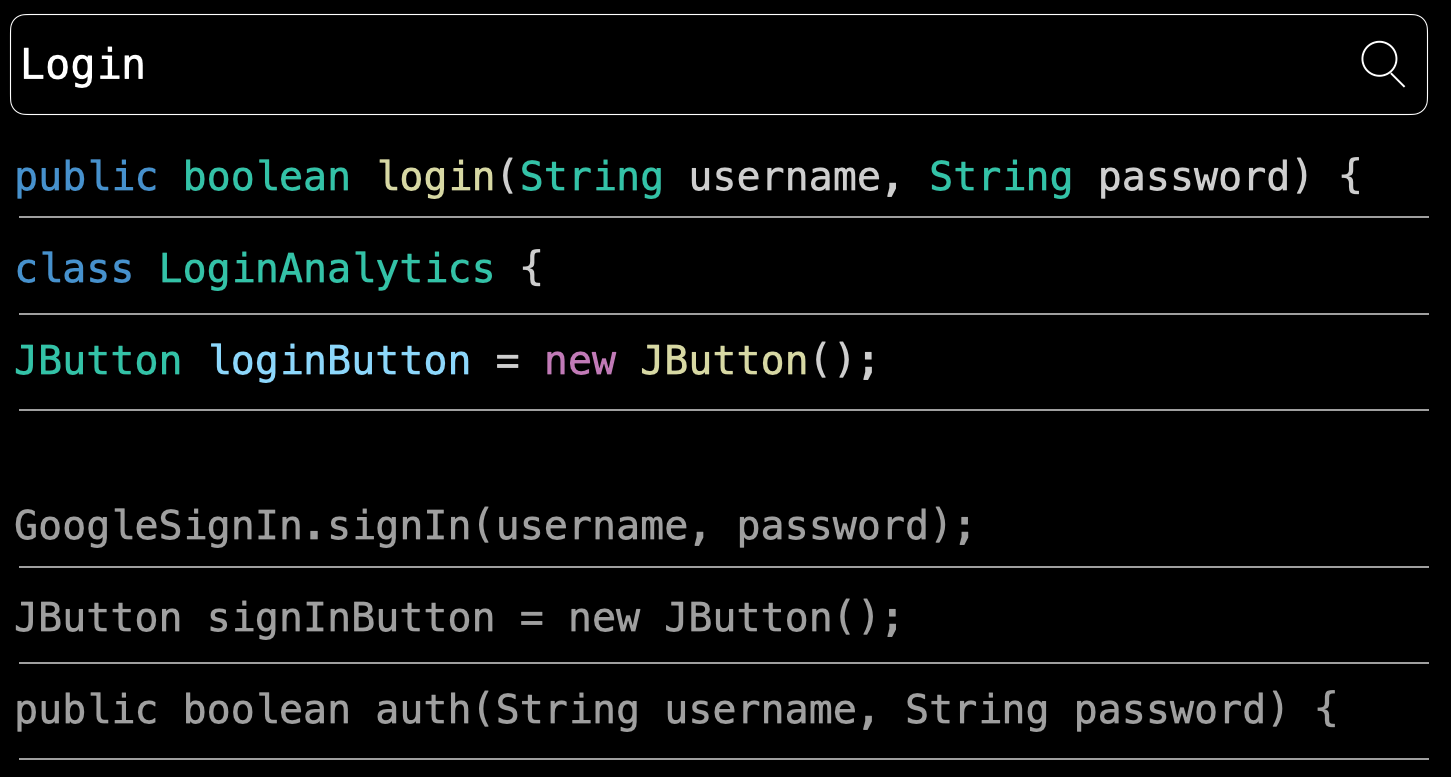
\includegraphics[width=0.8\columnwidth, height=0.4\columnwidth]{./imagens/intro/login-search.png}
  \smallcaption{Fonte: Autor}
  \label{fig:intro:login-search}
\end{figure}

Conforme visto no exemplo da Figura \ref{fig:intro:login-search}, a busca feita com a \textit{query} \textit{login} retornou os três primeiros trechos de código-fonte, os quais continham a palavra \textit{login}. Entretanto, os três últimos trechos de código-fonte (em cinza) não foram encontrados pela busca em questão, embora também sejam relacionados ao mesmo processo de autenticação do usuário no sistema.

Para mitigar esse problema de \textit{term mismatch} na busca de código, técnicas de \gls{nlp}, como \textit{query expansion} \cite{Nie2016QueryEB}, modelo booleano \cite{lv2015codehow} e, mais recentemente, modelos \textit{transformers} (como o \textit{CodeBERT} \cite{Feng2020CodeBERTAP}) vem sendo aplicados. Tais modelos \textit{transformers} se tornaram o estado da arte em busca de código-fonte utilizando linguagem natural pelo fato destes serem capazes de adicionar informações semânticas às buscas \cite{Guo2021GraphCodeBERTPC}. Isso significa que tais modelos compreendem, além das informações textuais contidas no trecho de código, informações semânticas sobre o código-fonte, como quais tarefas este realiza.

Para realizar o treinamento de tais modelos \textit{transformers}, normalmente é utilizado uma estrutura chamada par código-fonte/descrição ou par código-fonte/comentário. Tal estrutura contém tanto um trecho de código-fonte, escrito em linguagem de programação, quanto um trecho, escrito em linguagem natural, descrevendo as tarefas realizadas por tal código-fonte \cite{Gu2021CRaDLeDC} \cite{Yao2019CoaCorCA}. Um exemplo de par código-fonte/descrição pode ser encontrado na Figura \ref{fig:intro:code-description-pair}.

\begin{figure}[H]
  \centering
  \caption{Exemplo de um par código-fonte/descrição}
  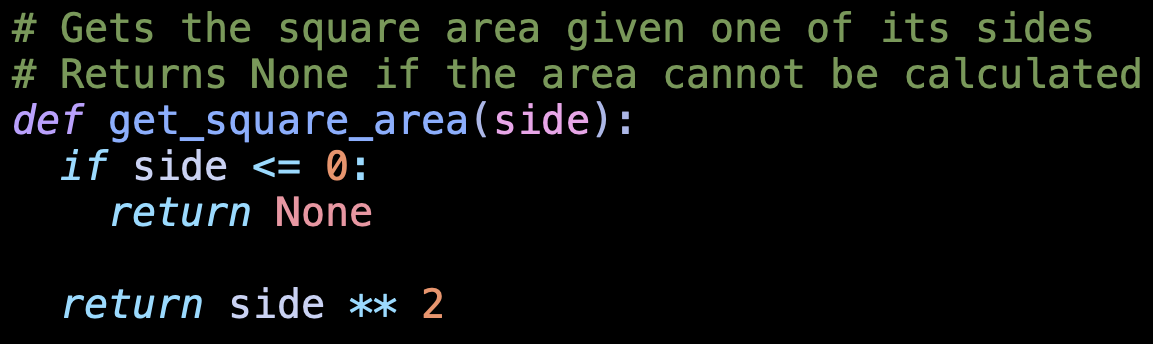
\includegraphics[width=\textwidth,keepaspectratio=true]{./imagens/intro/code-desc-pair.png}
  \smallcaption{Fonte: Autor}
  \label{fig:intro:code-description-pair}
\end{figure}

Na Figura \ref{fig:intro:code-description-pair}, há um trecho de código-fonte que realiza determinadas tarefas, e outro trecho em cinza, escrito em inglês (linguagem natural), descrevendo as tarefas realizadas pelo código-fonte em questão. Com isso, observa-se que o problema de busca de código-fonte lida com dois domínios de linguagem: o primeiro é o da linguagem natural, o qual contempla tanto a descrição do código-fonte quanto os termos de busca fornecidos pelo usuário. Já o segundo domínio refere-se às linguagens de programação, nas quais são escritos os trechos de códigos-fonte que serão buscados.

Entretanto, trabalhos como \textcite{Gu2018DeepCS} criam representações vetoriais (chamadas de \textit{embeddings}) tanto dos trechos de código-fonte quanto de suas descrições e das \textit{queries} do usuário. Com isso, ao comparar a similaridade entre os vetores gerados, estes sistemas inferem a semelhança entre a \textit{query} e determinados trechos de código-fonte trabalhando apenas em um domínio, a saber, no domínio vetorial dos \textit{embeddings}.

\section{Objetivo}
Com isso, o objetivo desse trabalho é utilizar uma rede \gls{mlp} para determinar a similaridade entre dois \textit{embeddings}, gerados por redes \textit{transformers}, de dois domínios diferentes: linguagem natural e linguagem de programação.

\section{Organização do trabalho}
O presente trabalho está organizado da seguinte forma: no capítulo \ref{chp:relatedWorks} é apresentado um retrato do estado da arte das áreas que o presente trabalho abrange, como busca de código e modelos \textit{transformers}. O capítulo \ref{chp:concepts} contém os principais conceitos teóricos abordados no presente trabalho. O capítulo \ref{chp:methodology} apresenta, em detalhes, a metodologia aplicada durante o desenvolvimento do trabalho. No capítulo \ref{chp:experiments} são descritos os experimentos realizados durante o estudo. Os resultados destes experimentos podem ser encontrados no capítulo \ref{chp:results}, enquanto o capítulo \ref{chp:discussions} apresenta algumas discussões sobre os resultados apresentados, bem como possíveis trabalhos futuros relacionados ao presente estudo. Por fim, o capítulo \ref{chp:conclusao} apresenta as conclusões do presente estudo.

\chapter{TRABALHOS RELACIONADOS}
\label{chp:relatedWorks}

O presente capítulo apresenta o estado da arte em relação à ferramentas de busca de código-fonte. Os trabalhos apresentados nesses capítulo estão ordenados em três seções: estudos relacionados à busca de código-fonte, ferramentas de busca de código-fonte e ferramentas de busca de código-fonte baseados em modelos \textit{transformers}. Todas as seções apresentam os estudos ordenados em ordem cronológica de publicação. Por fim, é apresentada também uma conclusão sobre os trabalhos citados neste capítulo.

\section{Estudos relacionados à busca de código-fonte}
\textcite{Sadowski2015HowDS} realizaram um estudo empírico entre desenvolvedores da empresa Google para analisar padrões de busca de código. O estudo foi realizado utilizando duas ferramentas: um questionário com cinco perguntas, que era apresentado ao usuário sempre que este acessava o repositório interno da empresa; e a coleta de registros (logs) gerados por uma ferramenta de busca de código, utilizada pelos usuários do estudo. Os resultados mostraram que programadores realizam, em média, cinco sessões de busca de código, com doze consultas por sessão, por dia de trabalho. Além disso, tais consultas são, geralmente, relacionadas aos seguintes pontos: uso de API; o que o código faz; porque o código está falhando; onde o código está localizado. Como trabalhos futuros, os autores apontam algumas áreas que não foram contempladas pelo estudo em questão, como a qualidade dos resultados da busca e de que forma os resultados da busca são utilizados pelo usuário. 

\textcite{Akbar2019SCORSC} estudaram a combinação de \glspl{cam} com a semântica dos vetores de palavras obtidos pelo algoritmo \textit{word2vec}. Com isso, os autores compararam as sequências de palavras de uma consulta em linguagem natural, e de um código-fonte. Utilizando as métricas \textit{MAP}, \textit{Precision@k} e \textit{Recall@k}, além das bases de dados \textit{BUGLinks} e \textit{iBUGS}, o estudo em questão obteve melhoras entre $6\%$ e $30\%$ de acurácia na busca de código.

\textcite{Heyman2020NeuralCS} estudaram o impacto que códigos anotados tem em modelos de busca de código. Segundo os autores, um código anotado é um trecho de código com descrições de sua intenção em linguagem natural. Durante o estudo, foram utilizados os modelos de busca de código \gls{ncs} e \gls{unif}, além das bases de dados \textit{CoNaLa}, \textit{StaQC} \cite{Yao2018StaQCAS} e SO-DS, as quais contém códigos em \emph{Python}. Como \emph{benchmark}, foram utilizadas as métricas \textit{recall@3}, \textit{recall@10} e \gls{mrr}. Ao se utilizar código anotado, obteve-se uma melhora de $20.6\%$ no \gls{mrr}, $23,9\%$ no \textit{recall@3} e $26,4\%$ no recall@10, em comparação aos métodos de busca que não utilizam código anotado. Por fim, os autores acreditam que tais melhorias poderão ser notadas mesmo como outras linguagem de programação (como Java, por exemplo), caso seja aplicado o uso de código anotado nos modelos de busca.

\textcite{Yan2020AreTC} observaram dificuldades em se comparar métodos de busca de código, como a falta de uma bases de dados em comum para comparação de dois métodos de busca. Diante disso, os autores realizaram um estudo empírico para comparação de dois tipos de métodos de busca de código a partir de consultas em linguagem natural. Os dois tipos de método em questão são: métodos baseados em \gls{ir}, e baseados em \gls{dl}. Para tanto, os autores criaram uma base de dados com códigos Java, chamada \textit{CosBench}, e utilizaram essa base para comparar quatro métodos de busca \gls{ir} e dois métodos \gls{dl}. Por fim, os resultados mostraram que os métodos baseados em aprendizagem profunda são mais adequados para consultas relacionadas à reutilização de código, enquanto métodos baseados em recuperação de informação são mais adequados para consultas relacionadas à resolução de \emph{bugs} e usos de determinadas \glspl{api}. Como trabalhos futuros, os autores levantam que a intenção da consulta feita pelo programador possa ser inferida automaticamente, de forma a ajudá-lo a encontrar o melhor método de busca para sua consulta.

\textcite{Salza2021OnTE} estudaram a aplicação de modelos \textit{transformers} em busca de código. Para tanto, os autores utilizaram dados do \textit{Stack Overflow} e do \textit{GitHub} para gerar bancos de dados de diversas linguagens de programação, como \textit{JavaScript}, \textit{Java} e \textit{Python}. Além disso, utilizou-se um modelo \textit{transformer} baseado no \gls{bert}, e as métricas \gls{mrr}, \textit{Aroma} e \textit{Top-k}. Com isso, o estudo concluiu que a transferência de conhecimento, possibilitada pelos modelos \textit{transformers}, é um método efetivo para melhorar a performance de busca de código em redes neurais. Entretanto, pelo fato dos modelos \textit{transformers} demandarem uma quantidade significativa de recursos computacionais, o estudo sugere a utilização de outros modelos de busca de código, como \textit{Apache Lucene}, para bases de dados pequenas. Por fim, no estudo em questão os autores utilizaram o modelo \gls{bert}, que analisou o código como uma sequência de \textit{tokens}. Entretanto, os autores sugerem que os resultados obtidos pelo BERT seriam melhores caso este fosse capaz analisar a estrutura do código, como a \gls{ast} por exemplo.

\textcite{Sun2022OnTI} propuseram um sistema para redução de ruído em bases de dados de busca de código. Tal sistema consiste em dois filtros subsequentes: um filtro sintático e um semântico. Nos experimentos, os autores utilizam o modelo de busca \gls{deepcs} para comparação, bem como as métricas \gls{mrr} e \textit{Answered@k} (com k = 1), além de dados disponíveis em \cite{Husain2019CodeSearchNetCE} e no GitHub. Com isso, observou-se uma média de $19,2\%$ e $21,3\%$ nas métricas \gls{mrr} e \textit{Answered@k}, respectivamente.

\section{Ferramentas de busca de código-fonte}

\textcite{lv2015codehow} notaram que as ferramentas de busca de código existentes tinham dificuldades com consultas em linguagem natural. Por isso, os autores propuseram a \textit{CodeHow}: uma ferramenta de busca de código que utiliza o modelo booleano extendido. Este modelo avalia a similaridade do texto da consulta com a documentação do código, a fim de ranquear os resultados da consulta em questão. Os autores conduziram o estudo com vinte desenvolvedores e estagiários da empresa Microsoft. Ao final, a \textit{CodeHow} obteve $0,794$ utilizando a métrica \textit{Precision@1}, e $0,867$ com a métrica \gls{mrr}. Tais resultados superaram as ferramentas existentes durante o período do estudo, como Ohloh e Apache Lucene. Contudo, os autores levantaram que, como a \textit{CodeHow} não consegue compreender os significados semânticos da consulta e do código, algumas consultas retornaram resultados incorretos. Um exemplo é a consulta "converter uma cor de RGB para HSV", para a qual a \textit{CodeHow} retornava resultados relevantes à consulta "converter uma cor de HSV para RGB".

\textcite{Gu2018DeepCS} propuseram uma rede neural profunda, chamada \textit{CODEnn}, capaz de relacionar trechos de código com consultas em linguagem natural. Além disso, os autores criaram uma ferramenta de busca de código (\gls{deepcs}), baseada na \textit{CODEnn}, como prova de conceito do estudo em questão. Para relacionar linguagem natural com código, a \textit{CODEnn} aprende as representações vetoriais do par código/descrição, de forma que um trecho de código é relacionado à uma consulta em linguagem natural utilizando o vetor gerado pela consulta. Utilizando este método, os autores obtiveram resultados de busca de código melhores do que ferramentas como Apache \textit{Lucene} e \textit{CodeHow}. Por fim, como trabalhos futuros, os autores pretendem investigar mais aspectos de códigos-fontes, como estruturas de controle, a fim de melhorar a representação de semânticas de alto nível do código-fonte.

\textcite{Cambronero2019WhenDL} analisaram o uso de modelos de aprendizado supervisionado e não supervisionado dentro do contexto de busca de código. Para tanto, os autores criaram uma plataforma comum de testes, e utilizaram \textit{benchmarks} como \gls{mrr}, além de criarem um modelo supervisionado, chamado \gls{unif}, o qual consiste em uma variação de um modelo \gls{ncs} (não supervisionado). Nos testes, os autores obtiveram resultados melhores com modelos supervisionados do que com modelos não supervisionados. Com isso, os autores sugerem o uso modelos de aprendizagem mais simples (como o \gls{unif}) para sistemas de busca de código. Além disso, o estudo mostra que uma base de dados de treinamento que se assemelhe com consultas comuns dos usuário, provê melhorias significativas para todos os modelos supervisionados.

\textcite{Wan2019MultimodalAN} propuseram o modelo \gls{mman} para busca semântica de código. O \gls{mman} utiliza diversos outros modelos, como \gls{lstm}, \textit{Tree-LSTM} e \gls{ggnn}, para representar características do código-fonte. O estudo em questão comparou o \gls{mman} com outros métodos de busca de código (como \textit{CodeHow} e \gls{deepcs}) utilizando as métricas \textit{SuccessRate@k} e \gls{mrr}, além de dados disponíveis no \textit{Github} para criação da base de dados. Com isso, o \gls{mman} obteve os melhores resultados no estudo. Como trabalhos futuros, os autores planejam aplicar o \gls{mman} em outras tarefas de engenharia de software como sumarização de código e detecção de plágio em código-fonte.

\textcite{Yao2019CoaCorCA} propuseram um modelo de aprendizagem por reforço, chamado \gls{coacor}, o qual gera descrições (em linguagem natural) de código-fonte a fim de melhorar modelos de busca de código. Os testes do estudo foram realizados com a base de dados \textit{StaQC} \cite{Yao2018StaQCAS} e utilizando os modelos de busca de código \gls{deepcs} e \textit{CODEnn}, além do \gls{mrr} e \gls{bleu} como métricas para busca de código e geração de descrição, respectivamente. Os resultados mostraram que o \gls{coacor} foi capaz de gerar descrições úteis para trechos de código, e que tais descrições foram capazes de melhorar a performance dos modelos de busca testados.

\textcite{Li2020LearningCI} propuseram o \gls{cqil}, um modelo de busca de código que utiliza redes neurais convolucionais para encontrar relações léxicas e semânticas entre a consulta e o trecho de código. A fim de comparação, o estudo utilizou os modelos de busca \gls{deepcs}, \gls{unif}, Apache Lucene e \textit{CodeHow}, bem como as métricas \textit{map@k}, \textit{SuccessRate@k} e \gls{mrr}, além das base de dados \textit{CODEnn} e \textit{CosBench}. Os experimentos realizados mostraram melhora de performance em todas as métricas utilizadas. Além disso, os autores apontam que o \gls{cqil} também possui boa performance com bases de dados pequenas.

\textcite{Ye2020LeveragingCG} utilizaram geração de código para melhor correlacionar linguagem de programação e linguagem natural. Para tanto, o modelo proposto, chamado \gls{co3}, utiliza \textit{dual
learning} e \textit{multi-task learning}. Para os experimentos, os autores utilizaram o banco de dados \textit{StaQC} \cite{Yao2018StaQCAS}, o qual contém trechos de código das linguagens de programação \gls{sql} e \textit{Python}. Utilizando as métricas \gls{mrr} e \gls{ndcg}, os autores obtiveram $0,585$ e $0.682$ (respectivamente) para \gls{sql}, e $0,679$ e  $0,756$ para \textit{Python}. Como trabalhos futuros, os autores planejam explorar as interações entre as perdas de ranking para busca de código.

\textcite{Ling2020AdaptiveDC} propuseram um método de busca de código chamado \gls{adacs}. Este método divide o processo de aprendizagem em duas etapas: aprendizagem de \textit{embeddings} de domínio específico, e aprendizagem de combinações de padrões sintáticos. Isso possibilita ao \gls{adacs} se adaptar à novas palavras, específicas de determinado domínio, mesmo que estas não tenham sido aprendidas durante o treinamento. Para os experimentos, o estudo utilizou códigos escritos em \textit{Java} e disponíveis no \textit{Github} e métodos de busca de código como \textit{CodeHow} e \gls{deepcs}. Utilizando as métricas \gls{mrr} e \textit{hit@k}, o \gls{adacs} obteve resultados melhores em todas as comparações feitas no estudo. Por fim, dentre os possíveis trabalhos futuros, os autores planejam melhorar a eficiência de tempo do \gls{adacs} utilizando \textit{encoders} transformers.

\textcite{Xu2021TwoStageAM} propuseram um modelo de busca de código chamado \gls{tabcs}, o qual consiste em um modelo de atenção de duas etapas: a primeira extrai dados semânticos tanto do código quanto da consulta, enquanto a segunda etapa detecta as relações semânticas entre código e consulta, a fim de aprender representações melhores dessas duas entidades. Em comparação com os modelos \gls{carlcscnn}, \gls{deepcs} e \gls{unif}, o \gls{tabcs} obteve uma melhora de $18\%$, $70\%$ e $12\%$ no \gls{mrr} respectivamente. Como trabalhos futuros, os autores planejam incorporar outras características do código-fonte, como estruturas de controle de fluxo, a fim de melhorar a representação do código-fonte.

\textcite{Bui2021SelfSupervisedCL} propuseram um modelo de aprendizagem auto-supervisionado contrastante para modelagem de código-fonte chamado \textit{Corder}. Este modelo pode ser usado tanto para produzir a rotulação de dados, as quais são aplicadas em sumarização de código, quanto para produzir representações  vetoriais de código-fonte, utilizadas em tarefas de busca de código. Para os experimentos relacionados à busca de código a partir de texto (\textit{text-to-code}), utilizou-se a base de dados disponível em \cite{Gu2018DeepCS}. Para comparação, foram utilizadas as métricas \textit{Precision@k} e \gls{mrr}, além dos modelos transformer, \gls{nbow}, \gls{tbcnn} e \gls{bilstm}. Em todos os experimentos realizados, os autores observaram melhoras no resultados dos modelos que utilizaram o \textit{Corder}, em relação aos que não utilizaram.

\textcite{Gu2021CRaDLeDC} propuseram um modelo de representação de código-fonte chamado \gls{cradle}. Este modelo combina as informações semânticas e de dependência contidas na instrução do código, a fim de gerar uma representação vetorial unificada para cada par código/descrição. O estudo utilizou as bases de dados \textit{CodeSearchNet} \cite{Husain2019CodeSearchNetCE} e \textit{Code2Sec}. Além disso, utilizou-se as métricas \textit{R@k} e \gls{mrr}, e os modelos de busca de código \textit{CODEnn}, \gls{unif} e \gls{nbow} para comparação de performance. Dos resultados, obteve-se melhoras em todas as métricas com a utilização do \gls{cradle}. Como trabalhos futuros, os autores pretendem incorporar, ao treinamento da rede, conhecimentos externos ao código, como documentação de \glspl{api}, a fim de melhorar a representação semântica do código-fonte.

\textcite{Liu2021GraphSearchNetEG} desenvolveram o modelo de busca de código \textit{GraphSearchNet}. Este modelo utiliza uma \gls{gnn} bidirecional para representar as informações estruturais tanto das consultas quanto do código-fonte. Além disso, o modelo proposto utiliza um módulo de atenção múltipla para suplementar as dependências globais dos grafos gerados. O \textit{GraphSearchNet} foi comparado com diversos modelos de busca (como \gls{deepcs}, \gls{unif} e \gls{nbow}), utilizando as métricas \textit{SuccessRate@k}, \gls{ndcg} e \gls{mrr}, além da base de dados \textit{CodeSearchNet} \cite{Husain2019CodeSearchNetCE}, utilizando os dados linguagens \textit{Python} e \textit{Java} para o estudo em questão. Por fim, a \textit{GraphSearchNet} obteve resultados melhores em todas as métricas utilizadas. Além disso, a \textit{GraphSearchNet} obteve uma performance melhor na linguagem \textit{Python}. Isso se deu, segundo os autores, porque \textit{Python} possui recursos gramaticais mais simples e uma distância semântica (\textit{semantic gap}) menor, quando comparada ao \textit{Java}.

\textcite{Zeng2021deGraphCSEV} notaram que as ferramentas de busca de código que utilizam aprendizagem de máquina são limitadas pelas técnicas de representação e modelagem do código-fonte. Portanto, os autores propuseram a \gls{degraphcs}, capaz de converter código-fonte em grafos de fluxo baseado em variáveis, a fim de modelar a semântica do código de forma mais precisa do que \gls{ast}. Como trabalhos futuros, os autores apontam otimizações para remoção de informações redundantes nos grafos gerados.

\textcite{Du2021IsAS} perceberam que um trecho de código contém diferentes características, como lógica de negócio e comunicação com \textit{hardware}, de forma que seria difícil um único modelo representar todas essas dimensões. Com isso, os autores propuseram a \textit{MuCoS}, uma arquitetura de aprendizagem multimodal para busca semântica de código. Nessa arquitetura, ao invés de um módulo de aprendizagem para descrever todas as características do código, há múltiplos módulos de aprendizagem, um para cada característica. Depois, os autores utilizam técnicas de aprendizagem por agrupamento (\textit{ensemble learning}) para combinar todos os módulos. Para os testes, os autores utilizam a base de dados \textit{CodeSearchNet} \cite{Husain2019CodeSearchNetCE} e as métricas \textit{SuccessRate@k} (com $k=1$, $k=5$ e $k=10$) e \gls{mrr}. Utilizando tais métricas, o \textit{MuCoS} obteve $0,750$, $0,843$, $0,860$ e $0,793$, respectivamente. O segundo melhor modelo testado no estudo, \textit{CodeBERT}, obteve $0,642$, $0,792$, $0,825$ e $0,708$, respectivamente. Por fim, os autores planejam implementar um módulo de seleção para ajudar a escolher modelos de aprendizagem específicos para determinada busca.

\textcite{Ling2021DeepGM} propuseram um modelo para busca semântica de código-fonte chamado \gls{dgms}. Esse modelo representa tanto textos em linguagem natural quanto trechos de códigos com uma estrutura unificada de grafos. O estudo avaliou o \gls{dgms} utilizando as bases de dados \textit{FB-Java} e \textit{CSN-Python}. Além disso, os autores compararam o \gls{dgms} com os modelos \gls{nbow}, \gls{deepcs}, \gls{unif} e \textit{CAT} \cite{Haldar2020AMA}, utilizando as métricas \gls{mrr} e \textit{SuccessRate@k}. Por fim, o estudo mostrou que o \gls{dgms} obteve resultados consideravelmente melhores do que os outros modelos, nas duas métricas utilizadas no estudo em questão. Além disso, os autores planejam explorar outras formar de construir grafos de texto e código para outras linguagem de programação, como C\#.

\textcite{Sun2022CodeSB} propuseram um modelo de busca de código chamado \textit{TranCS}. Primeiro, o \textit{TranCS} utiliza uma técnica de tradução de código para linguagem natural baseada em contexto. Depois, o \textit{TranCS} utiliza uma função de mapeamento a fim gerar \textit{embeddings} tanto para as traduções quanto para as buscas de código. Tanto a técnica de tradução quanto a função de mapeamento foram desenvolvidas pelos autores.
Com isso, os autores compararam o \textit{TranCS} com os modelos \gls{deepcs} e \gls{mman}, utilizando a base de dados de \cite{Husain2019CodeSearchNetCE} e a métrica \gls{mrr}. Os resultados mostraram que o \textit{TranCS} obteve melhoras de $49,31\%$ a $66,50\%$ em relação aos outros modelos utilizados no estudo. Como trabalhos futuros, os autores citaram a construção de representações para longos trechos de código (acima de 20 linhas, segundo os autores).

\textcite{Shi2022EnhancingSC} desenvolveram um modelo para busca de código que utiliza aprendizagem multimodal contrastiva e \textit{soft data augmentation} chamado \textit{CoCoSoDa}. A \textit{soft data augmentation} é obtida mascarando e substituindo alguns \textit{tokens} na sequências de código para gerar trechos de código que são similares, mas que não necessariamente preservam a relação semântica entre o par código/consulta. Os experimentos do estudo utilizaram as métricas \gls{mrr} e \textit{SuccessRate@k}, e a base de dados \textit{CodeSearchNet} \cite{Husain2019CodeSearchNetCE}. Para comparação de performance, foram utilizados os modelos \gls{nbow}, redes neurais convolucionais, redes neurais recorrentes bidirecionais e \textit{SelfAtnn}. Os experimentos também testaram a aplicação do CoCoSoDa para melhorar a performance de modelos de atenção. Os modelos de atenção testados foram \textit{RoBERTa}, \textit{CodeBERTa},
\textit{CodeBERT} e \gls{graphcodebert}. Os resultados mostraram que o \textit{CoCoSoDa} obteve uma performance melhor do que os modelos testados. Além disso, os modelos de atenção que utilizam o CoCoSoDa também apresentaram melhoras de performance. Como trabalhos futuros, os autores pretendem convidar desenvolvedores para avaliar a relação semântica entre trechos de código e consultas em linguagem natural.

\textcite{Wang2022EnrichingQS} propuseram \gls{quecos}, um modelo de aprendizagem por reforço para busca de código. O estudo utilizou as bases de dados \textit{CodeSearchNet} \cite{Husain2019CodeSearchNetCE} e \textit{SOTorrent}. Além disso, para comparação utilizou-se as métricas \textit{SuccessRate@k} e \gls{mrr}, e os modelos de busca de código \gls{deepcs}, \gls{unif}, \textit{OCoR} e \textit{CodeBERT}. Dos resultados, nota-se que o \gls{quecos} obteve resultados melhores do que os modelos comparados, em todas as métricas consideradas no estudo. Como trabalhos futuros, os autores planejam utilizar bases de dados maiores para o treinamento, além de incorporarem grafos de conhecimento externos para melhorar a semântica das buscas.

\textcite{Gu2022AcceleratingCS} propuseram um modelo de busca de código, baseado em \textit{deep hashing} e classificação de código, chamado \gls{coshc}. O estudo utilizou dois bancos de dados de código em \textit{Python} e \textit{Java}, ambos providos por \cite{Feng2020CodeBERTAP}. Para comparação, foram utilizados os modelos \gls{unif}, \gls{rnn}, \textit{CodeBERT}, \textit{CodeBERTa} e \textit{GraphCodeBERT}, além da métrica \textit{SuccessRate@k}. Os resultados mostraram que o \gls{coshc} foi melhor em comparação ao modelos \gls{unif} e \gls{rnn}, mas obteve resultados iguais ou piores na maioria dos testes com \textit{CodeBERT}, \textit{CodeBERTa} e \textit{GraphCodeBERT}.

\textcite{Cheng2022CSRSCS} propuseram um modelo de busca de código chamado \gls{csrs}, o qual consiste de três partes principais: um módulo de \textit{embedding} com núcleos de convolução para extrair \textit{embeddings} n-gramas de consultas e códigos; um módulo para medir as correspondências léxicas das consultas; e um módulo baseado em atenção para capturar a correlação semântica entre consulta e código. Utilizando a métrica \gls{mrr}, e a base de dados utilizada em \cite{Gu2018DeepCS}, o \gls{csrs} obteve melhora de $33,77\%$ e $18.53\%$ em relação aos modelos \gls{deepcs} e \gls{carlcscnn}. Como trabalhos futuros, os autores consideram estudar formas de melhorar a combinação dos módulos do \gls{csrs}, além de incorporar conhecimento externo (como \gls{ast} ou documentação de \gls{api}) ao treinamento do \gls{csrs}.

\section{Ferramentas de busca de código-fonte baseada em modelos \textit{transformers}}

\textcite{Chu2019AGA} propôs um sistema para busca de código que combina aprendizagem de máquina baseada em grafos com modelos \emph{transformer}, além de modelos tradicionais de busca como \textit{ElasticSearch} (ferramenta de busca baseada no Apache \textit{Lucene}). O sistema em questão aplicou \emph{embeddings} hiperbólicos e clusterização de grafos aos dados da base \emph{CodeSearchNet} \cite{Husain2019CodeSearchNetCE}, a fim de incorporar a estrutura de grafos presente nos repositórios de código aos modelo de busca testados. Com isso, foram testados os seguintes modelos de busca: \gls{nbow}; \textit{ElasticSearch}; \textit{ElasticSearch} com clusterização de grafos. Utilizando a métrica \gls{ndcg}, comumente utilizada para avaliar mecanismos de busca, obteve-se $0,190$ com o \gls{nbow}, $0,196$ com \textit{ElasticSearch} e $0,208$ com o \textit{ElasticSearch} com clusterização de grafos. Por fim, dentre as melhorias sugeridas pelos autores está a utilização de outros modelos neurais no lugar do \textit{ElasticSearch}, combinados com o modelo de grafos proposto.

\textcite{Feng2020CodeBERTAP} propuseram o \textit{CodeBERT}, um modelo bimodal para linguagem de programação e linguagem natural. O \textit{CodeBERT} utiliza uma arquitetura baseada no modelo \gls{bert}. Porém, o \textit{CodeBERT} é capaz de aceitar tanto dados bimodais (par código/linguagem natural) quanto dados unimodais (apenas código). Dados bimodais geralmente são usados para tarefas de busca de código, enquanto dados unimodais para geração de código. Com o \textit{CodeBERT}, os autores conseguiram resultados iguais ou, em alguns casos, melhores do que o estado da arte. As comparações foram feitas utilizando as métricas \gls{mrr} para busca de código e \gls{bleu} para geração de código. Por fim, como trabalhos futuros, os autores apontam a incorporação de \gls{ast} nas fases de pré-treino.

\textcite{Wang2020TranS3AT} propuseram o $TranS^3$, o qual consiste em um modelo, baseado em redes \textit{transformer}, para integração de sumarização de código e busca de código. O $TranS^3$ é capaz de gerar comentários para determinado trecho de código. Com isso, utilizando os comentários gerados, o $TranS^3$ consegue melhorar o treinamento para busca de código, relacionando assim trechos de código com linguagem natural. A fim de avaliar a performance de busca de código, o estudo utilizou as métricas \gls{mrr}, \textit{SuccessRate@k} e \gls{ndcg}, bem como diversos modelos de busca de código como \gls{deepcs}, \textit{Hybrid-DeepCom} e \gls{coacor}. Dos resultados, observa-se que o $TranS^3$ obteve performance semelhante ou melhor do que todos os modelos comparados, tanto na tarefa de busca de código quanto de sumarização de código.

\textcite{Guo2021GraphCodeBERTPC} desenvolveram o \gls{graphcodebert}: um modelo \textit{transformer} pré-treinado para linguagens de programação, que considera a estrutura inerente do código-fonte. Para tanto, ao invés de usar estruturas sintáticas de código como a \gls{ast}, o \gls{graphcodebert} utiliza o \textit{data flow}. O \textit{data flow} consiste em uma representação de código-fonte, a qual é menos complexa do que \gls{ast}, e contém informações sobre as relações entre as variáveis utilizadas no código. O estudo testou o \gls{graphcodebert} em tarefas relacionadas à linguagem de programação, incluindo busca de código a partir de linguagem natural. Para esta tarefa em específico, os autores utilizaram a métrica \gls{mrr}, o banco de dados \textit{CodeSearchNet} \cite{Husain2019CodeSearchNetCE} e sete modelos de busca de código, incluindo \gls{nbow}, \gls{birnn}, \textit{RoBERTa}, \textit{CodeBERTa} e \textit{CodeBERT}. Em todas as comparações, os autores notaram que o \gls{graphcodebert} obteve resultados melhores na tarefa de busca de código a partir de linguagem natural.

\textcite{Chai2022CrossDomainDC} propuseram um modelo chamado \gls{cdcs}. Diferente do \textit{CodeBERT} que precisa ser treinado na linguagem de código alvo, o \gls{cdcs} é pré-treinado com uma grande base de dados de determinada linguagem, como \textit{Java} ou \textit{Python}. Então, utilizando o algoritmo de meta-aprendizagem \textit{MAML}, o \gls{cdcs} se adapta a linguagem alvo que, no caso do estudo em questão, foi \gls{sql} e \textit{Solidity}. Os experimentos do estudo foram avaliados utilizando as métricas \gls{mrr} e top-k, e mostraram que o \gls{cdcs} atingiu melhoras significativas no domínio de busca de código, quando comparado com outros modelos como \textit{CodeBERT} e \textit{GPT2}. Por fim, os autores pretendem investigar a aplicação do \gls{cdcs} com outras linguagem de programação, além de aplicar o \gls{cdcs} em outras tarefas de engenharia de software.

\section{Conclusões do Capítulo}
O gráfico da Figura \ref{fig:related-datasets} mostra as bases de dados utilizadas nos estudos analisados. Nota-se que a grande maioria das bases utiliza dados disponíveis ou no \textit{Github} (\textit{CodeSearchNet} e \textit{CosBench}) ou no \textit{Stack Overflow} (\textit{StaQC}). O fácil acesso, grande volume de dados e a forma como os dados estão estruturados podem ser explicações para o uso dessas duas fontes de dados. Inclusive, essa estruturação é especialmente relevante no caso do \textit{Stack Overflow}. Além das respostas dos usuários normalmente conterem tanto um trecho de código-fonte quanto sua explicação em linguagem natural, há também um sistema de votação, fazendo com que os trechos de código-fonte mais relevantes e menos relevantes para a pergunta inicial sejam, indiretamente, anotados pelos usuários da plataforma. A saber, a base de dados de \textit{queries} utilizada no experimento 3, descrito na seção \ref{sec:experiments:experiment-3}, também utiliza anotações feitas manualmente.


\begin{figure}[H]
    \centering
    \caption{Bases de dados utilizadas}
    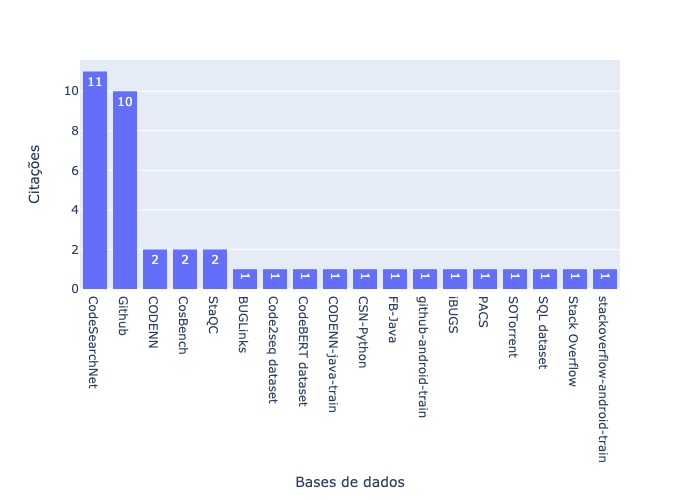
\includegraphics[width=1.0\columnwidth, height=0.6\columnwidth]{./imagens/trabalhos-relacionados/databases.png}
    \smallcaption{Fonte: Autor}
    \label{fig:related-datasets}
\end{figure}

O gráfico da Figura \ref{fig:related-metrics} mostra as métricas utilizadas nos estudos em questão. Nota-se que \gls{mrr} e \textit{SuccessRate@k} foram as métricas mais utilizadas para o problema de busca de código. Por conta disso, utilizou-se as métricas \gls{mrr} no experimento 2, descrito na seção \ref{sec:experiments:experiment-2}.
\begin{figure}[H]
    \centering
        \caption{Métricas utilizadas}
        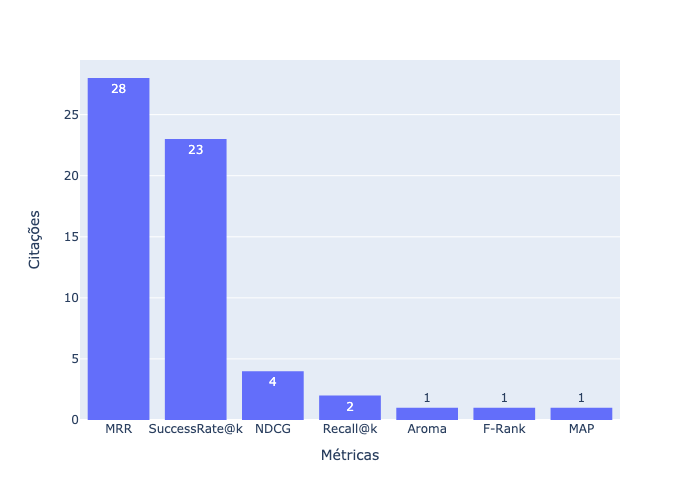
\includegraphics[scale=0.5]{./imagens/trabalhos-relacionados/ir_metrics.png}
        \smallcaption{Fonte: Autor}
        \label{fig:related-metrics}
\end{figure}

A Figura \ref{fig:related-baselines} mostra os modelos de busca de código utilizados como base de comparação nos estudos em questão. Nota-se que a maioria dos modelos utilizam redes neurais profundas, com exceção do \gls{unif}, \textit{Apache Lucene} e \textit{ElasticSearch}. Além disso, nota-se o uso extensivo de modelos \textit{transformers} baseados em \gls{bert}, como \textit{CodeBERT}, \textit{RoBERTa} e \textit{GraphCodeBERT} - por isso foram selecionados modelos \textit{transformers} baseados em \gls{bert} ou \textit{RoBERTa} no presente estudo, conforme descrito no capítulo \ref{chp:methodology}. Uma possível explicação para o uso de modelos \textit{transformers} é a eficiência de tais modelos quando comparados com outras técnicas como busca textual ou redes neurais profundas.
\begin{figure}[H]
    \centering
        \caption{Modelos de comparação utilizados}
        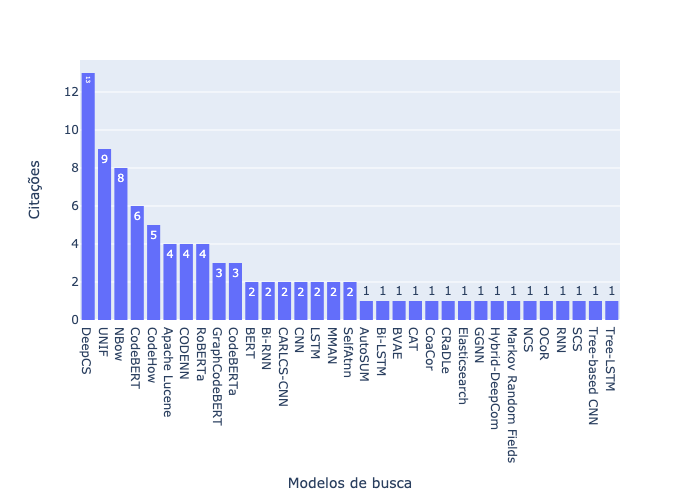
\includegraphics[scale=0.5]{./imagens/trabalhos-relacionados/baselines.png}
        \smallcaption{Fonte: Autor}
        \label{fig:related-baselines}
\end{figure}

Portanto, a fim de determinar qual o melhor modelo apresentado, conclui-se que não é possível realizar tal comparação utilizando os resultados apresentados em seus respectivos estudos. Isso porque, apesar dos experimentos utilizarem as mesmas métricas de busca, os resultados dependem de fatores específicos dos estudos em questão, como a base de dados utilizada.

\chapter{Conceitos}
\label{chp:concepts}
Nesse capítulo serão apresentados os principais conceitos que serão utilizados ao longo da metodologia apresentada.

\section{Sistemas de Busca de Código-Fonte}
Na literatura, encontra-se diferentes técnicas para busca de código-fonte. Antes, porém, é importante definir alguns termos comumente utilizados nessa área de busca de código-fonte. \textit{Query} é a entrada do sistema - os termos introduzidos pelo usuário para realizar uma busca. A intenção do usuário é o que este quer buscar, e que será expressa através da \textit{query}. Sistemas de busca de código-fonte, por sua vez, consistem em encontrar trechos de código-fonte relevantes à \textit{query} inserida pelo usuário. A Figura \ref{fig:concepts:code-search-structure} mostra um exemplo de busca de código-fonte.

\begin{figure}[H]
    \centering
    \caption{Exemplo de busca de código-fonte}
    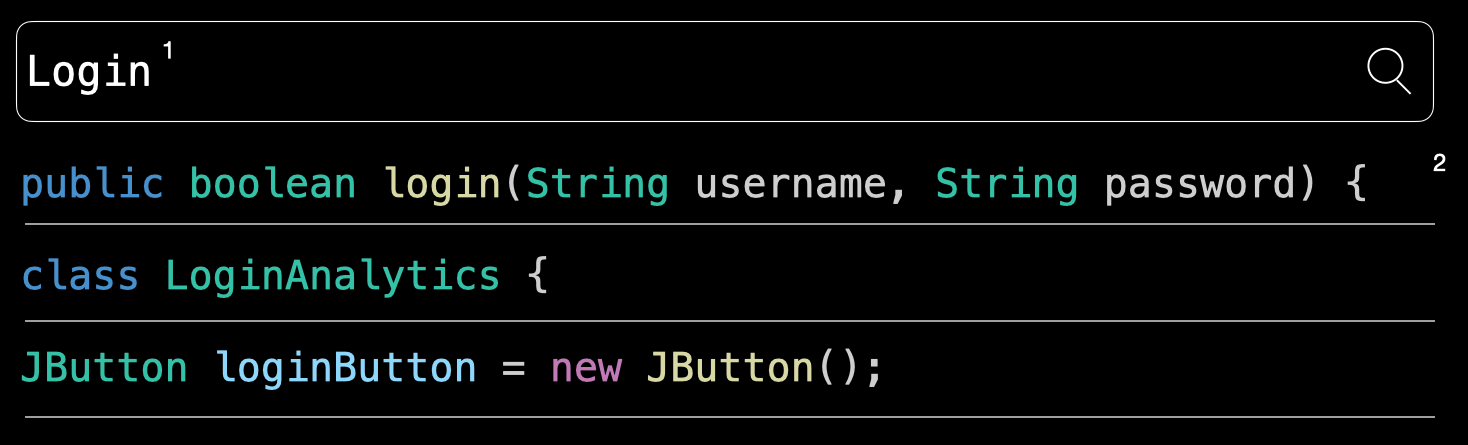
\includegraphics[width=\textwidth,keepaspectratio=true]{imagens/conceitos/code-search-structure.png}
    \smallcaption{Fonte: Autor}
    \label{fig:concepts:code-search-structure}
\end{figure}

Na Figura \ref{fig:concepts:code-search-structure}, a intenção do usuário era encontrar trechos de código-fonte relacionados a autenticação em determinado sistema. A \textit{query} utilizada para essa busca foi \textit{login} (1) e, para essa \textit{query}, foram encontrados três trechos de código-fonte (2).

Dito isso, \textcite{Grazia2022CodeSA} realizaram uma extensa revisão nos trabalhos da área e, segundo os autores, três fatores são considerados ao desenvolver sistemas de busca de código-fonte. São estes:
\begin{itemize}
  \item Facilidade de uso: o usuário deve ser capaz de criar \textit{queries} sem treinamento ou conhecimento prévio do sistema.
  \item Expressividade: dada quaisquer intenção do usuário, este deve ser capaz de expressá-la por meio de \textit{queries}.
  \item Precisão: as \textit{queries} devem ser capazes de expressar a intenção do usuário com o mínimo de ambiguidade.
\end{itemize}

\textit{Queries}, como dito anteriormente, são a interface do usuário com o sistema. Em busca de código-fonte, há diferentes formas de \textit{queries}, dependendo do sistema. 
Trabalhos como \cite{NGUYEN2017CombiningWW}, \cite{Chen2018ANF} e \cite{Du2021IsAS} utilizam \textit{queries} em linguagem natural, como português ou inglês. Este formato de \textit{queries} proporciona facilidade de uso e expressividade, enquanto perde em precisão da \textit{query} pelo fato de haver ambiguidades inerentes às linguagens naturais. Sistemas como \textit{Google}, \textit{Stack Overflow} e \textit{Github} utilizam esse formato de \textit{query}.

Outros trabalhos, como \textcite{Zhou2018SLAMPARC}, \textcite{Fujiwara2019CodetoCodeSB} e \textcite{Mukherjee2020SearchingAD}, utilizam \textit{queries} no formato de código-fonte. Uma possível \textit{query} desses sistemas seria apenas a declaração de uma função em linguagem de programação. Com isso, o sistema seria responsável por procurar trechos de código-fonte que servissem como corpo dessa função. \textit{Queries} neste formato provêm facilidade de uso, mas a precisão e expressividade variam de acordo com a intenção do usuário \cite{Grazia2022CodeSA}. Por fim, tais sistemas são utilizados, principalmente, para sugestões de código-fonte enquanto o usuário escreve o código.

\textcite{Martie2015CodeExchangeSR} e \textcite{Sivaraman2019ActiveIL} propuseram uma linguagem de busca estruturada, similar às linguagens de banco de dados como \gls{sql} para busca de código-fonte. Para encontrar códigos-fonte com os trechos \textit{import math} e \textit{def sum(a, b):}, uma possível \textit{query} válida nesses sistemas seria \textit{'import math' AND 'def sum(a,b):'}. Com essa estrutura de \textit{queries}, tais sistemas provem alta precisão e expressividade, em detrimento da facilidade de uso, pelo fato do usuário precisar aprender uma nova linguagem para realizar as buscas.

Por outro lado, trabalhos como \textcite{Reiss2009SemanticsbasedCS} e \textcite{Jiang2018ResearchPS} recebem a entrada e saída esperadas como \textit{queries}, e buscam códigos-fonte que, dada tal entrada produza a saída correspondente. Por exemplo: dada a entrada esperada 'nOmE' e a saída esperada 'nome', o sistema irá buscar códigos-fonte que produzam tal saída, dada tal entrada. Tal formato de \textit{query} provê facilidade de uso, mas são necessárias muitas \textit{queries} para se alcançar expressividade e, principalmente, precisão. Ainda, tais sistemas possuem aplicações em metodologias de desenvolvimento de \textit{software} como \textit{test-driven development}, onde o usuário primeiro escreve os testes para depois implementar a funcionalidade. A ideia é que, dado os testes (que possuem valores de entrada e saída definidos), o sistema de busca de código-fonte encontre quais trechos de código satisfazem tais testes.

Além disso, há diferentes técnicas de busca de código-fonte na literatura. Trabalhos como \textcite{Lu2015QueryEV} e \textcite{Li2016RelationshipawareCS}, por exemplo, utilizam uma técnica chamada \textit{query expansion}. Nela, dada uma \textit{query} o sistema realiza mais de uma busca com termos similares aos da \textit{query}, a fim de melhorar os resultados da busca. 

Depois, trabalhos como \textcite{Mitra2018AnIT}, \textcite{Gu2018DeepCS} e \textcite{Sun2022CodeSB} utilizam técnicas de \textit{machine learning} no problema de busca de código-fonte a partir de linguagem natural. Durante o aprendizado, estes modelos geram \textit{embeddings} para dois domínios: de linguagem natural e de código-fonte. O primeiro, geralmente são extraídos textos de comentários e documentações, os quais descrevem as tarefas realizadas por determinado código-fonte. O segundo corresponde ao código-fonte em si. Com isso, a similaridade entre a \textit{query} e o código-fonte se dá no espaço vetorial dos \textit{embeddings}.

De forma semelhante, trabalhos recentes como \textcite{Feng2020CodeBERTAP} e \textcite{Guo2021GraphCodeBERTPC} utilizam modelos \textit{transformers} para aprender as relações semânticas entre linguagem natural (da \textit{query} e das descrições dos códigos-fontes presentes nas bases de treinamento) e do código-fonte. Atualmente, tais sistemas são o estado da arte na área de busca de código-fonte.

\section{Aprendizagem de máquina em Processamento de Linguagem Natural}

A aplicação de técnicas de aprendizagem de máquina tem melhorado significativamente o estado da arte da área de processamento de linguagem natural, conforme visto em modelos como \gls{nbow}, \gls{deepcs} e \gls{bert}.

Porém, modelos de aprendizagem de máquina trabalham com números ao invés de texto. Com isso, para utilizar esses modelos dentro da área de \gls{nlp}, utiliza-se um conjunto de técnicas chamado \textit{word embedding}. Tais técnicas criam representações vetoriais a partir de \textit{tokens}, os quais podem então servir como entrada para modelos de aprendizagem de máquina. Desse conjunto de técnicas, destaca-se a família de algoritmos \textit{Word2Vec} \cite{Mikolov2013EfficientEO} \cite{Mikolov2013DistributedRO}.

Os \textit{tokens} utilizados pelo \textit{word embedding} são gerados por algoritmos chamados tokenizadores. Estes algoritmos geram \textit{tokens} a partir de determinado corpus ou bases textuais \cite{Mielke2021BetweenWA}. \textit{Tokens} são unidades menores dos textos, como por exemplo palavras, morfemas ou símbolos específicos do \textit{tokenizador} - portanto, os \textit{tokens} gerados dependem do tokenizador. Em modelos \textit{transformers}, os tokenizadores mais utilizados são \gls{bpe} e \textit{WordPiece}.

O \gls{bpe} inicialmente cria uma lista com todas as palavras distintas do corpus de treinamento. A partir dessa lista, um vocabulário é gerado com todas as letras distintas - e textos com palavras que não estavam no corpus de treinamento serão substituídos pelo token \textit{unknown} (desconhecido). Aqui, vale ressaltar que modelos transformers como \gls{gpt2} e \gls{roberta} utilizam uma variação do \gls{bpe} chamada \textit{byte-level} \gls{bpe}, a qual utiliza \textit{bytes} ao invés das letras em formato Unicode, eliminando assim a necessidade do \textit{token} '\textit{unknown}'.

A partir do vocabulário inicial, o \gls{bpe} itera sobre todo o corpus de treinamento para determinar a frequência com que os \textit{tokens} de seu vocabulário ocorrem. Então, são gerados pares (daí o nome \textit{byte-pair}) contendo o \textit{token} e sua frequência no corpus de treinamento. Ao fim, o \gls{bpe} concatena os dois \textit{tokens} dos pares mais frequentes nessa iteração, a fim de criar um novo \textit{token} em seu vocabulário. Tais relações entre \textit{tokens}, aprendidas a partir de suas frequências no corpus de treinamento, são chamadas de regras de \textit{merge}. Por fim, vale notar que, a cada iteração, é adicionado um novo \textit{token} ao vocabulário do tokenizador. E a a quantidade de iterações que o tokenizador fará, e portanto o tamanho de seu vocabulário, é determinada pelo usuário.

O \textit{WordPiece} segue praticamente os mesmos passos do \gls{bpe}, com algumas diferenças da implementação. Inicialmente, o \textit{WordPiece} também gera um vocabulário a partir das palavras distintas que ocorrem no corpus de treinamento. A diferença em relação ao \gls{bpe} é que o \textit{WordPiece} adiciona um prefixo que indica a continuação de determinada palavra, às letras do vocabulário. Por exemplo, dada a palavra $frase$, os seguintes \textit{tokens} serão gerados: $[f, \#\#r, \#\#a, \#\#s, \#\#e]$. Outra diferença em relação ao \gls{bpe} é que, ao invés da frequência, os \textit{tokens} são combinados utilizando uma nota dada pelo \textit{WordPiece} a cada \textit{token}. Essa nota é computada utilizando a seguinte equação:
\begin{equation*}
y=\frac{f_{1,2}}{f_1 \times f_2}
\end{equation*}
Na equação acima, $y$ é a nota do \textit{token}, $f_{1,2}$ é a frequência do par de \textit{tokens}, $f_1$ a frequência do o primeiro \textit{token} do par e $f_2$ do segundo \textit{token}. Com isso, são gerados os \textit{tokens} de determinado corpus.

\section{Modelos de Atenção}
Modelos \textit{transformers}, como \gls{bert} e \gls{roberta}, utilizam algum tipo de modelo de atenção (ou mecanismo de atenção). Segundo \textcite{Vaswani2017AttentionIA}, atenção pode ser descrita como uma função de mapeamento entre um vetor \textit{query} $Q$ e um par chave-valor de vetores $K$ e $V$, respectivamente. \textcite{Vaswani2017AttentionIA} propõe uma função de atenção, chamada \textit{Scaled Dot-Product Attention}, a qual é descrita da seguinte forma \cite{Vaswani2017AttentionIA}:
\begin{equation*}
A(Q, K, V)= softmax(\frac{QK^T}{\sqrt{d_k}}) \times V
\label{eq:attention-equation}
\end{equation*}
Na qual $d_k$ é a dimensão do vetor $K$. Como o resultado do $softmax$ consiste em uma distribuição de probabilidades, a multiplicação vetorial do vetor resultante de $softmax(\frac{QK^T}{\sqrt{d_k}})$ com o vetor $V$ ativará alguma dimensão de $V$, indicando assim a atenção de $Q$ e $K$ em $V$, ou $A(Q, K, V)$.

Além disso, os modelos \textit{transformers} utilizam uma técnica chamada \textit{multi-head attention}. Nela, são realizadas projeções lineares dos vetores $Q$, $K$ e $V$, as quais foram aprendidas durante a fase de treinamento \cite{Vaswani2017AttentionIA}. Isso permite com que o modelo consiga observar, de forma conjunta, diferentes representações de determinado \textit{token} em diferentes posições do texto.

A arquitetura \textit{transformer} também prevê um vetor de posição para cada \textit{token}, para descrever sua posição no texto. Esse vetor é chamado \textit{positional encoding} e foi descrito por \textcite{Vaswani2017AttentionIA} da seguinte forma:
\begin{eqnarray*}
PE_{(pos, 2_i)} & = &\sin{\frac{pos}{10000^\frac{2_i}{d_m}}} \\
PE_{(pos, 2_(i+1))} & = & \cos{\frac{pos}{10000^\frac{2_i}{d_m}}}
\end{eqnarray*}
Na equação acima, $pos$ é a posição do \textit{token}, $d_m$ é a dimensão do modelo e $i$ é a dimensão atual, sendo que $0 \leq i \leq d$. Como as funções de seno e cosseno são periódicas, os valores gerados estarão entre $2\pi$ e $10000 \times 2\pi$. Com isso, o \textit{positional encoding} é capaz de descrever as posições absolutas e relativas de determinado \textit{token} no texto. Vale frisar que é possível descrever posições relativas neste modelo pois, dado um intervalo $k$ entre um \textit{token} e outro \textit{token} anterior, $PE_{pos+k}$ pode ser representado como função linear de $PE_{pos}$ \cite{Vaswani2017AttentionIA}.

Por fim, a Figura \ref{fig:transformer-architecture} mostra um diagrama com uma visão geral da arquitetura \textit{transformer}:

\begin{figure}[H]
    \centering
    \caption{Visão geral da arquitetura \textit{Transformer}}
    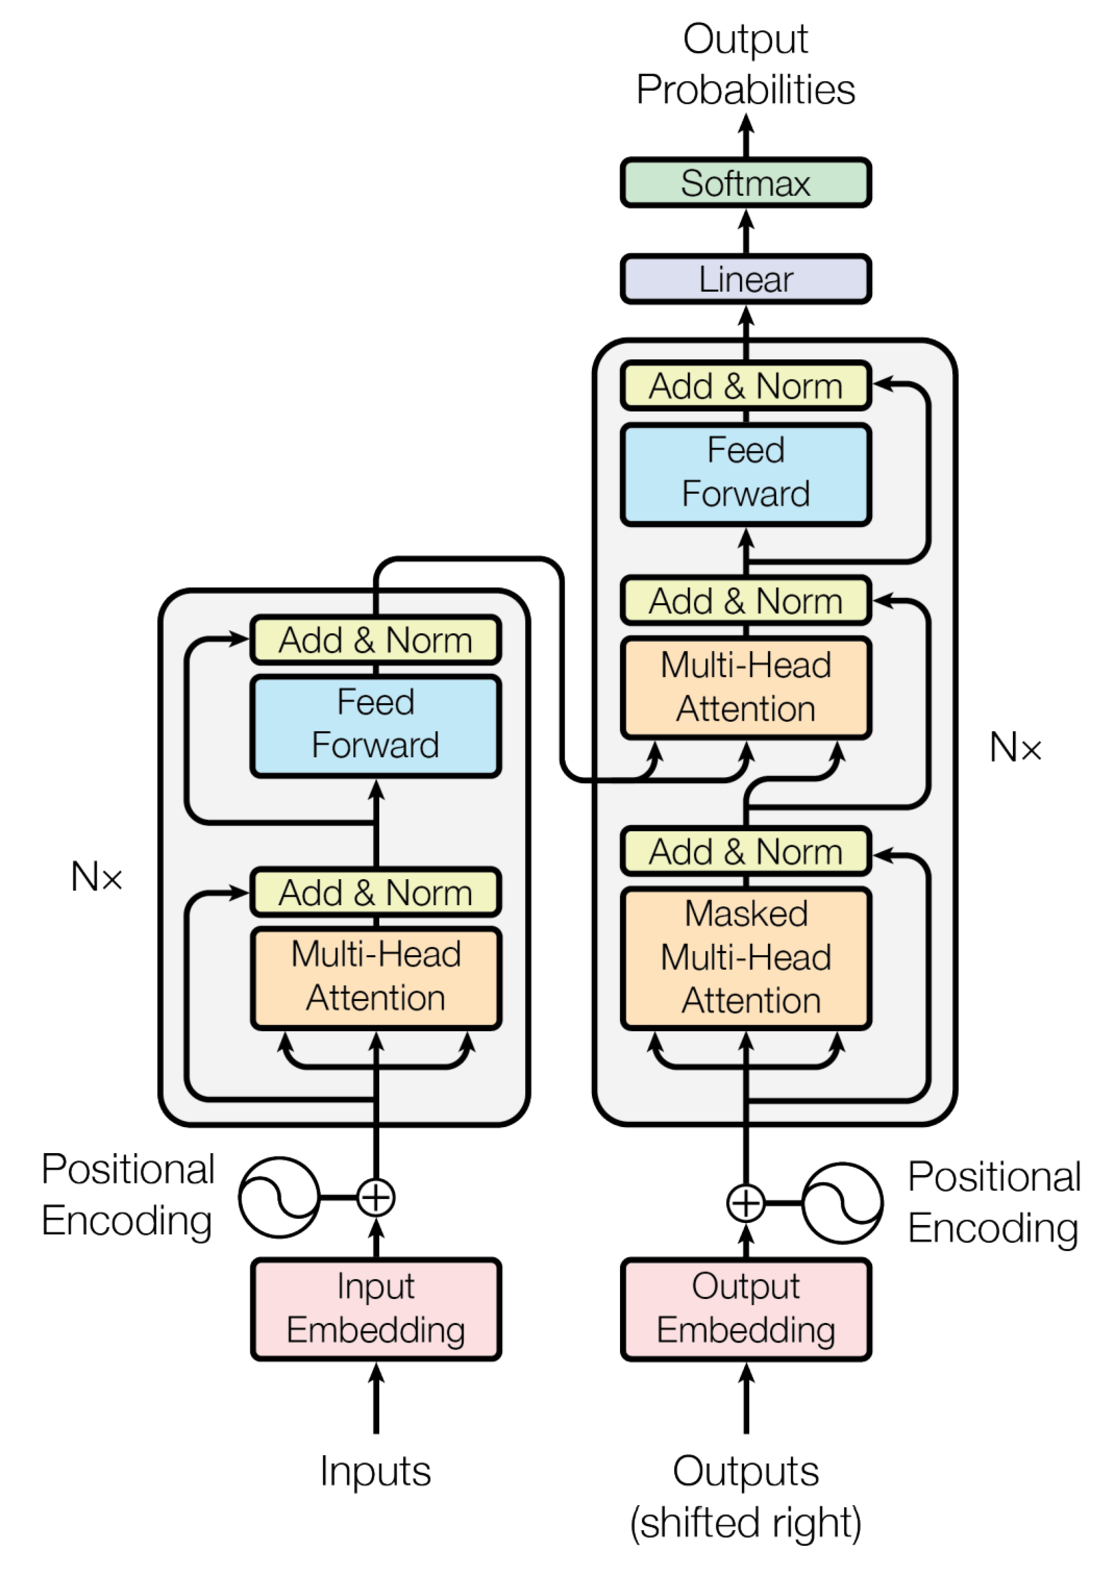
\includegraphics[scale=0.4]{imagens/conceitos/transformer-architecture.pdf}
    \smallcaption{Fonte: \cite{Vaswani2017AttentionIA}}
    \label{fig:transformer-architecture}
\end{figure}

Vale ressaltar que o \textit{pipeline} do lado esquerdo da Figura \ref{fig:transformer-architecture}, o qual recebe os \textit{embeddings} de entrada (\textit{input embeddings)}, é chamado de \textit{encoder}. E o \textit{pipeline} do lado direto da Figura \ref{fig:transformer-architecture} é chamado de \textit{decoder}.

Posteriormente, foi proposto o modelo \gls{bert} \cite{Devlin2019BERTPO}. Este consegue aprender, dado um \textit{token} do texto, o contexto tanto com os \textit{tokens} anteriores quanto com seus sucessores. Em outras palavras, o \gls{bert} aprende o contexto de forma bi-direcional. Como exemplo, dada a sentença "O menino foi passear na praia", modelos anteriores ao \gls{bert} processavam as palavras em sequência - primeiro "O", depois "menino", depois "foi" e assim por diante - até por conta dessa limitação que modelos como \gls{lstm} eram recursivos, a fim de guardar as informações de palavras previamente processadas; no exemplo em questão, para saber o contexto ao processar a palavra "foi", era necessário que estes modelos recorrentes salvassem as informações obtidas das palavras anteriores "O" e "menino".

Ainda, como o \gls{bert} utiliza apenas modelos de atenção, este consegue processar todas as palavras da frase em paralelo, aumentando drasticamente a performance de treinamento em relação aos modelos recorrentes, por exemplo. Porém, só os modelos de atenção não seriam suficientes para possibilitar o processamento em paralelo das palavras durante o treinamento do \gls{bert}, já que as posições das palavras na frase seriam perdidas. Por isso, além dos modelos de atenção, os modelos \textit{transformers} e, mais especificamente, o \gls{bert}, utilizam os \textit{positional embeddings} citados acima. Estes vetores descrevem tanto as posições relativas quanto absolutas de cada palavra na frase. Para fins didáticos, e utilizando a mesma frase "O menino foi passear na praia", considere que cada palavra é numerada a partir de zero - então, "O" estaria na posição 0, "menino" na posição 1 e assim por diante. Nesse caso, a posição absoluta da palavra "passear" seria 3 e a posição relativa à palavra "O" seria 2.

Além disso, também é possível pré treinar os modelos \textit{transformers}. Como tais modelos demandam muitos recursos computacionais durante seu treinamento, estes são geralmente pré-treinados com grandes quantidades de dados \textit{corpus} grande em determinado domínio. Por exemplo, dado o par código-fonte/comentário, tem-se dois domínios diferentes: código-fonte e linguagem natural, respectivamente. Portanto, utilizou-se dois modelos \textit{transformers} - um pré treinado com amostras de código-fonte, e outro com trechos de textos na lingua inglesa, conforme descrito no capítulo \ref{chp:experiments}. Com isso, não foi necessário treinar tais modelos de \textit{embedding} com a base de dados específica utilizada no presente estudo. 

Entretanto, é possível especializar ainda mais os modelos \textit{transformers} utilizando um processo chamado \textit{fine-tuning} onde, dado um domínio específico (como busca de código-fonte a partir de linguagem natural), tais modelos são treinados utilizando amostras específicas para o problema em questão, a fim de especializar os modelos \textit{transformers} no problema em questão e, com isso, aumentar sua performance. Como tal processo demanda muitos recursos, além de fugir do objetivo principal do presente estudo, o \textit{fine-tuning} não foi realizado para nenhum dos modelos \textit{transformers} citados no capítulo \ref{chp:experiments} \cite{Tay2021ScaleEI}.

\section{Métricas de Avaliação de Recuperação de Informação}
Dado uma lista de resultados para determinada busca, ordenados de maneira decrescente de relevância, o \gls{mrr} é um valor, entre 0 e 1, que representa em qual posição o resultado mais relevante estará na lista de resultados. Caso o \gls{mrr} seja 1, o resultado mais relevante estará (na maioria dos casos) em primeiro lugar na lista de resultados; se for 0.5, este estará na segunda posição e assim por diante \cite{Craswell2009}. Essa métrica é composta pela a média entre os resultados de várias buscas em determinada base de dados. Os valores individuais de cada busca são chamados de \gls{rr} e são calculados da seguinte forma:
\begin{equation*}
    RR_i=1/rank_i
\end{equation*}
Na equação acima, $rank_i$ é a posição de determinado resultado - se este estiver na primeiro posição, $RR=1/1=1$; se estiver na segunda, $RR=1/2=0.5$ e assim por diante. Com isso, tem-se que o \gls{mrr} é a média harmônica de todos os \glspl{rr} para a quantidade de buscas realizadas em determinada base de dados. Portanto, a fórmula do \gls{mrr} é dada por:
\begin{equation*}
    MRR = \frac{1}{|Q|} \times \sum_{i=1}^{|Q|} RR_i
\end{equation*}
Na qual $|Q|$ é a quantidade de buscas realizadas.

Por sua vez, \textit{SuccessRate@k} é um valor, entre 0 e 1, que representa a porcentagem de vezes que o resultado mais relevante da busca esteve nas primeiras $k$ posições da lista de resultados. Essa métrica é descrita pela fórmula \cite{Wan2019MultimodalAN}:
\begin{equation*}
    SuccessRate@k=\frac{1}{|Q|} \times \sum_{i=1}^{|Q|} \delta(FRank_i \geq k)
\end{equation*}
Na qual $\delta(x)$ é uma função que retorna 1 caso x for verdadeiro e 0 caso contrário. $FRank_i$ é a posição do resultado relevante na lista de resultados \cite{Raghothaman2016SWIMSW}. Por fim, vale ressaltar que autores tem utilizado outros nomes para se referir à essa mesma métrica. Citando alguns exemplos, \textcite{Ling2020AdaptiveDC} se refere à essa métrica como \textit{Hit@k}, \textcite{Bui2021SelfSupervisedCL} como \textit{Precision@k} e, ainda, \textcite{Gu2021CRaDLeDC} como \textit{R@k}. No presente estudo, entretanto, essa métrica será chamada de \textit{SuccessRate@k}.


\chapter{METODOLOGIA}
\label{chp:methodology}
\graphicspath{ {./imagens/metodologia} }

O objetivo do presente estudo é utilizar uma rede \gls{mlp} para determinar a similaridade entre dois \textit{embeddings} gerados por redes \textit{transformers}. A Figura \ref{fig:metodology-system_overview} mostra uma visão geral do sistema implementado durante este estudo. Neste capítulo, os módulos de cor azul representam processos relacionados ao código-fonte do par código-fonte/comentário, enquanto os módulos verdes representam processos relacionados ao comentário. Por fim, todos os módulos apresentados na Figura \ref{fig:metodology-system_overview} serão detalhados nas seções abaixo.

\begin{figure}[H]
    \centering
        \caption{Visão geral do sistema}
        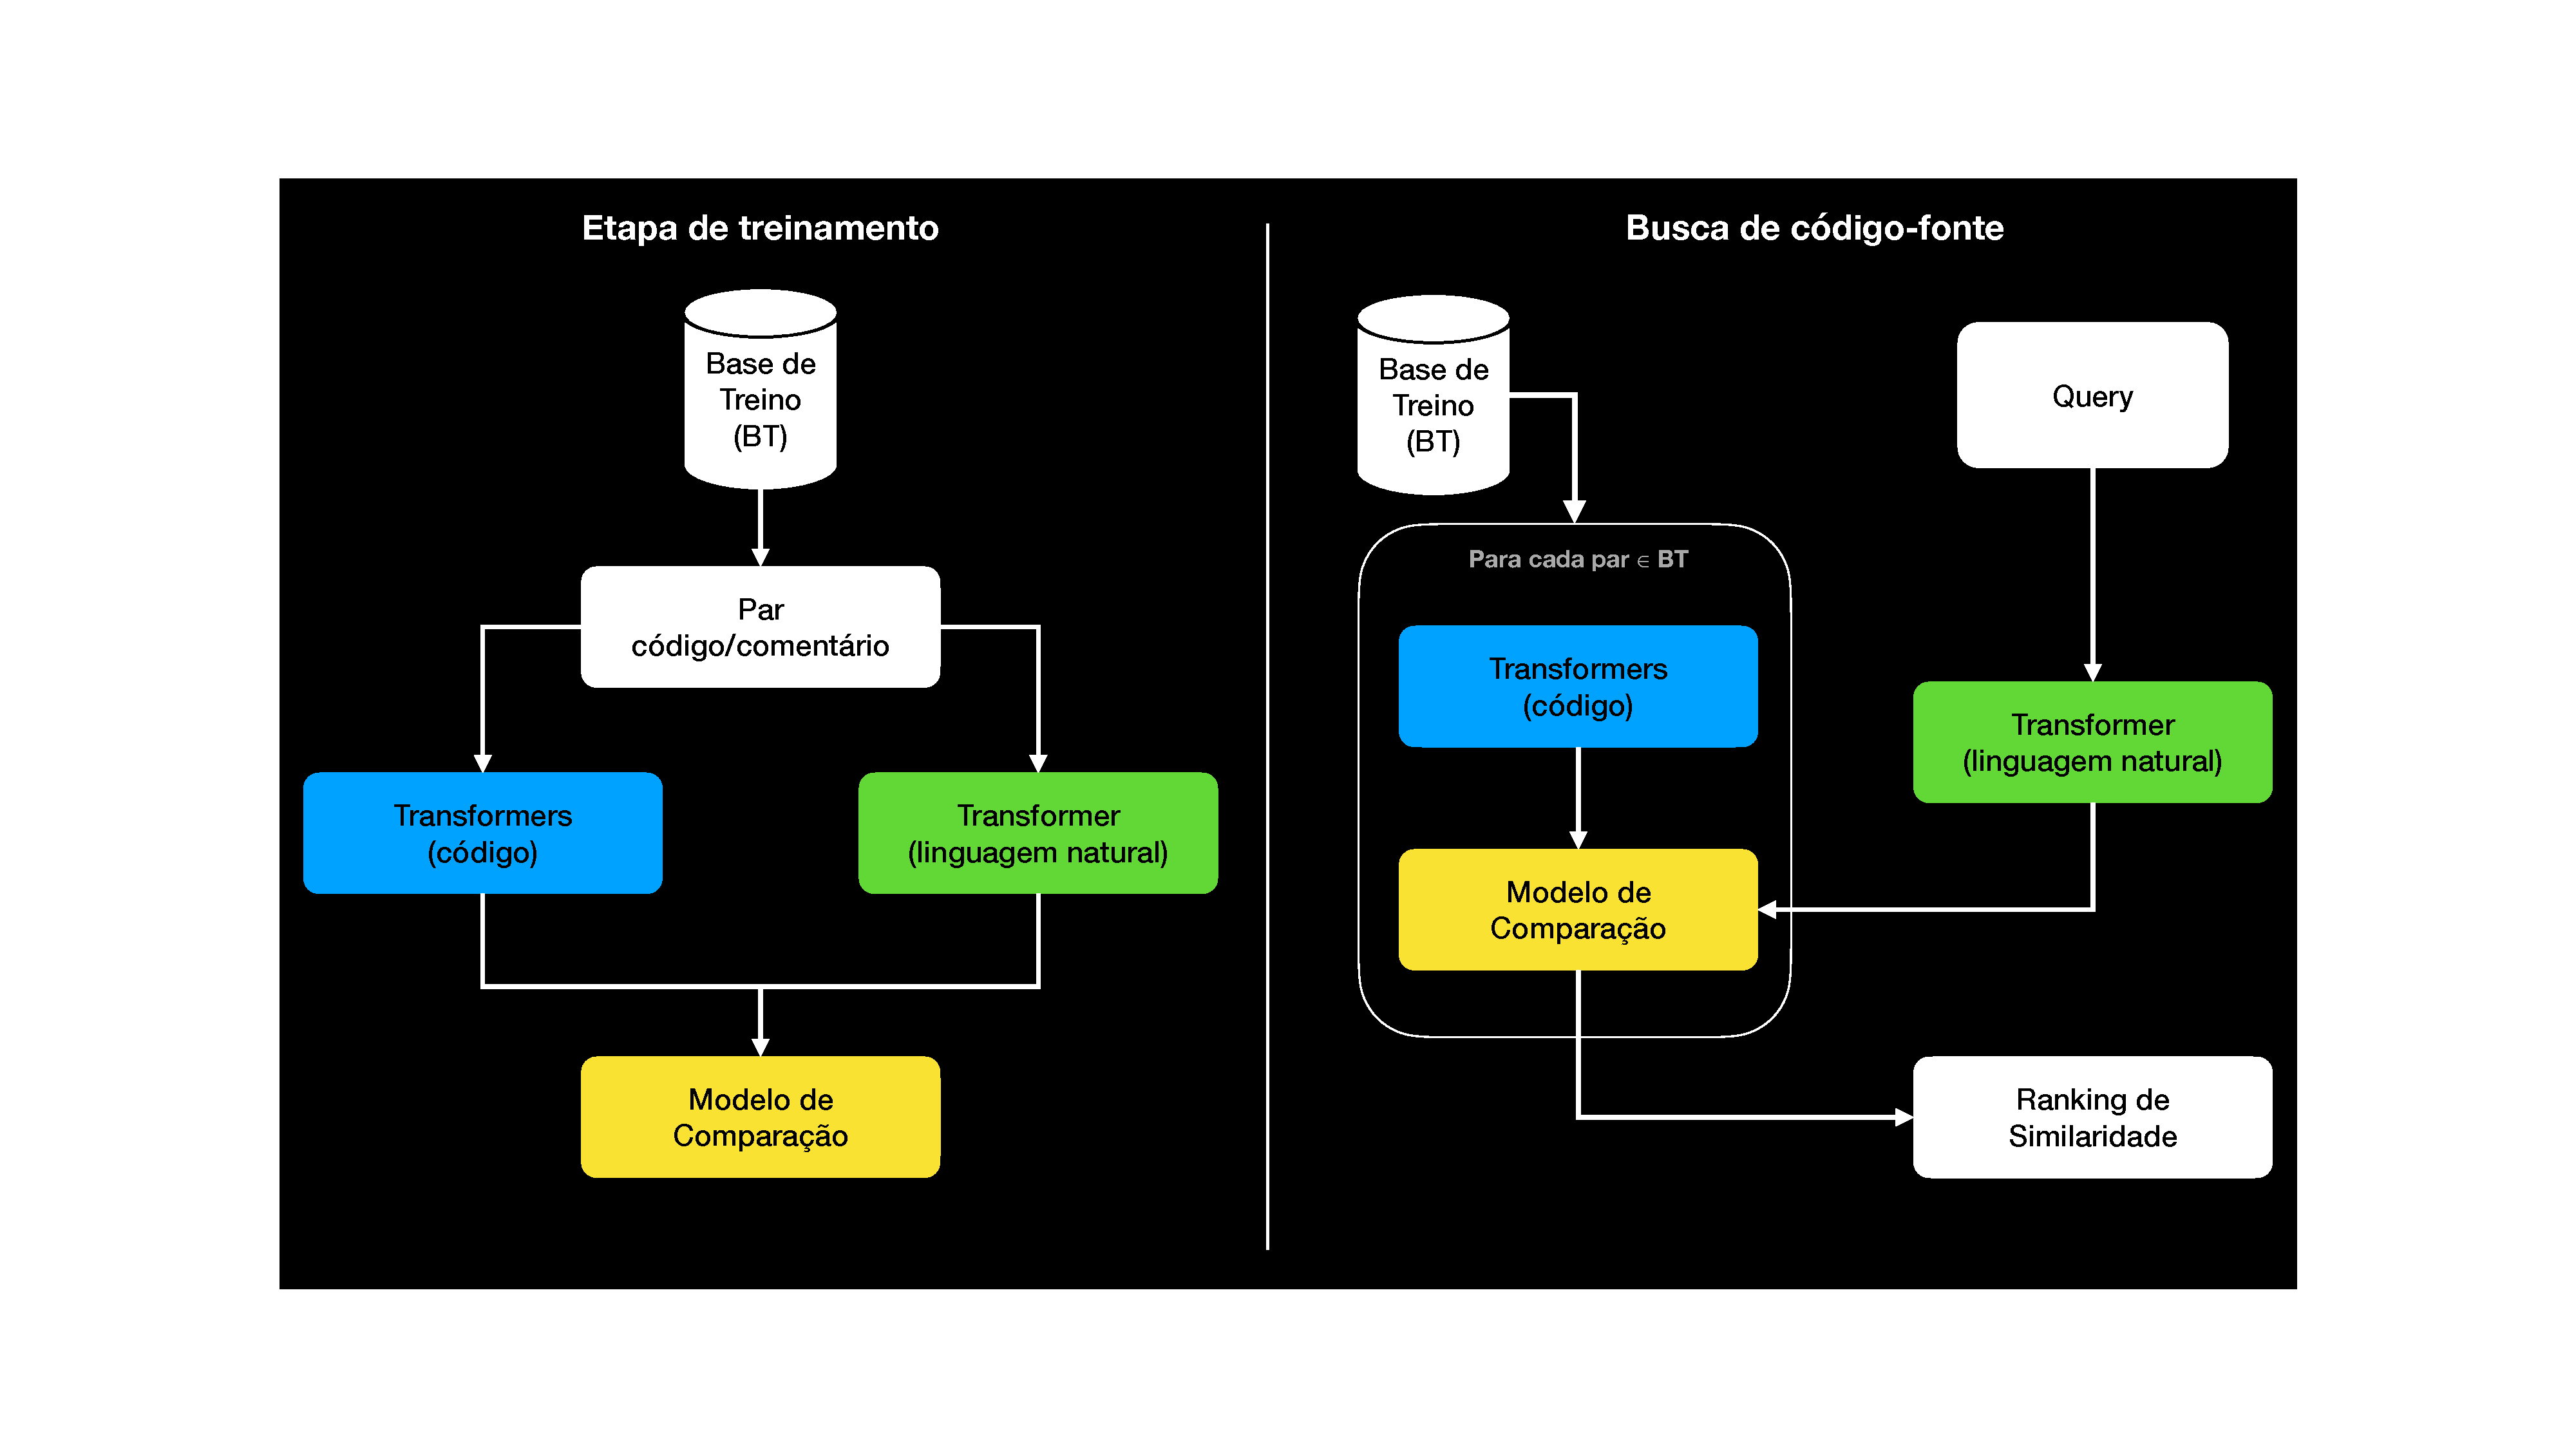
\includegraphics[scale=0.3]{system-overview.pdf}
        \smallcaption{Fonte: Autor}
        \label{fig:metodology-system_overview}
\end{figure}

\section{Base de treino}
Todos os experimentos serão realizados utilizando a base de dados \textit{CodeSearchNet} \cite{Husain2019CodeSearchNetCE}. Esta consiste em uma coleção de bases de dados e métricas voltadas ao problema de busca de código-fonte, totalizando dois milhões de pares código-fonte/comentário oriundos de repositórios de código aberto. A Figura \ref{fig:metodology-code-comment-pair} mostra um exemplo de par código-fonte/comentário.

\begin{figure}[H]
    \centering
        \caption{Par código-fonte/comentário}
        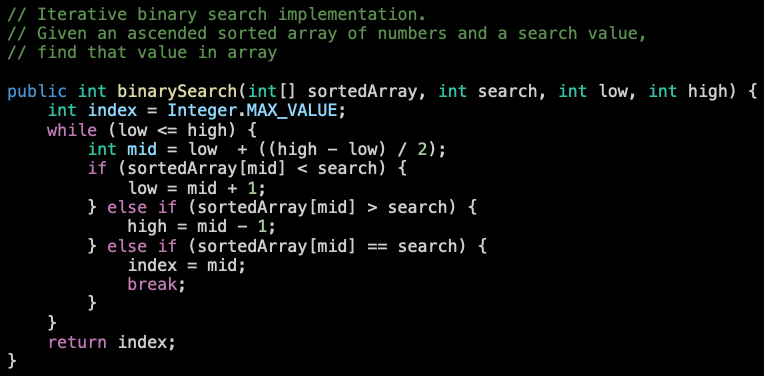
\includegraphics[scale=0.3]{code-comment-pair.png}
        \smallcaption{Fonte: Autor}
        \label{fig:metodology-code-comment-pair}
\end{figure}

Como é possível ver na Figura \ref{fig:metodology-code-comment-pair}, o código fonte é um trecho de código-fonte, em forma de função ou método de uma classe, o qual executa determinada tarefa. O comentário, por sua vez, é escrito em linguagem natural (no caso da base de dados em questão, em inglês), e descreve a tarefa executada pelo trecho de código-fonte correspondente.

Além disso, a base de dados contém pares com código-fonte das linguagens de programação \textit{Python}, \textit{Javascript}, \textit{Ruby}, \textit{Go}, \textit{Java} e \textit{PHP}. Neste trabalho, foram selecionados 2000 pares código-fonte/comentário com códigos-fonte na linguagem \textit{Python}.

Por fim, durante o desenvolvimento deste trabalho, a base de dados original \textit{CodeSearchNet} foi arquivada por seus criadores, não sendo possível mais acessá-la. Como alternativa, a base \textit{CodeSearchNet} foi migrada, por membros da comunidade, para um repositório no \textit{HuggingFace}\footnote{Disponível em https://huggingface.co/datasets/code\_search\_net}.


\section{Pré-processamento}
\label{sec:methodology:pre-processing}

Durante a migração do repositório original para o \textit{HuggingFace}, os autores deste novo repositório filtraram os pares originais da seguinte forma:
\begin{itemize}
    \item Códigos-fonte que não possuiam comentário foram removidos da base
    \item Comentários foram truncados até o primeiro parágrafo, a fim de evitar descrições muito longas de determinado código-fonte
    \item Pares que possuem comentários com menos que três \textit{tokens} foram removidos da base
    \item Funções construtoras e métodos padrão da linguagem de programação foram removidos da base. Como exemplo, podemos citar as funções \textit{init} ou \textit{str} da linguagem Python
\end{itemize}

\section{Base de pares de \textit{embeddings}}
\label{sec:methodology:encoders}
Após o pré-processamento, os modelos de \textit{transformers} serão responsáveis por gerar os \textit{word embeddings} tanto do código-fonte quanto do comentário correspondente. Para isso, foram escolhidos dois modelos: o \textit{all-mpnet-base-v2}, baseado em \gls{roberta}, para linguagem natural (comentário) e o \textit{flax-sentence-embeddings/st-codesearch-distilroberta-base}, baseado em DistilRoBERTa, para código-fonte. Apesar de modelos diferentes, ambos geram \textit{word embeddings} em um espaço vetorial de dimensão 768, além de serem pré-treinados utilizando, dentre outras bases de dados, a \textit{CodeSearchNet}.

Por fim, a Figura \ref{fig:metodology-db-embeddings} ilustra a criação da base de pares de \textit{embeddings} a partir de pares código-fonte/comentário. Como pode-se notar na imagem, para cada par código-fonte/comentário, é gerado um par de \textit{embedding} código-fonte/comentário. Essa nova base de pares de \textit{embeddings} é então salva em disco, para ser utilizada nas etapas seguintes. Durante a criação dos pares de \textit{embeddings}, não há nenhuma operação que altere a posição destes pares. Portanto, a associação entre o par original com o par de \textit{embedding} correspondente foi feita utilizando sua posição (\textit{index}) na base original. Com isso, dado que $i$ é a posição de determinado par na base de treinamento, para acessar os \textit{embeddings} do $par_i$ basta consultar a base de \textit{embeddings} na mesma posição $i$. Por fim, a geração da base de \textit{embeddings} acelerou tanto o treinamento do modelo de comparação (descrito na seção \ref{sec:methodology:embedding-comparator} deste capítulo) quanto os experimentos descritos no capítulo \ref{chp:experiments}, já que para ambas as etapas os pares de \textit{embeddings} já haviam sido gerados.

\begin{figure}[H]
    \centering
        \caption{Geração da base de pares de \textit{embeddings}}
        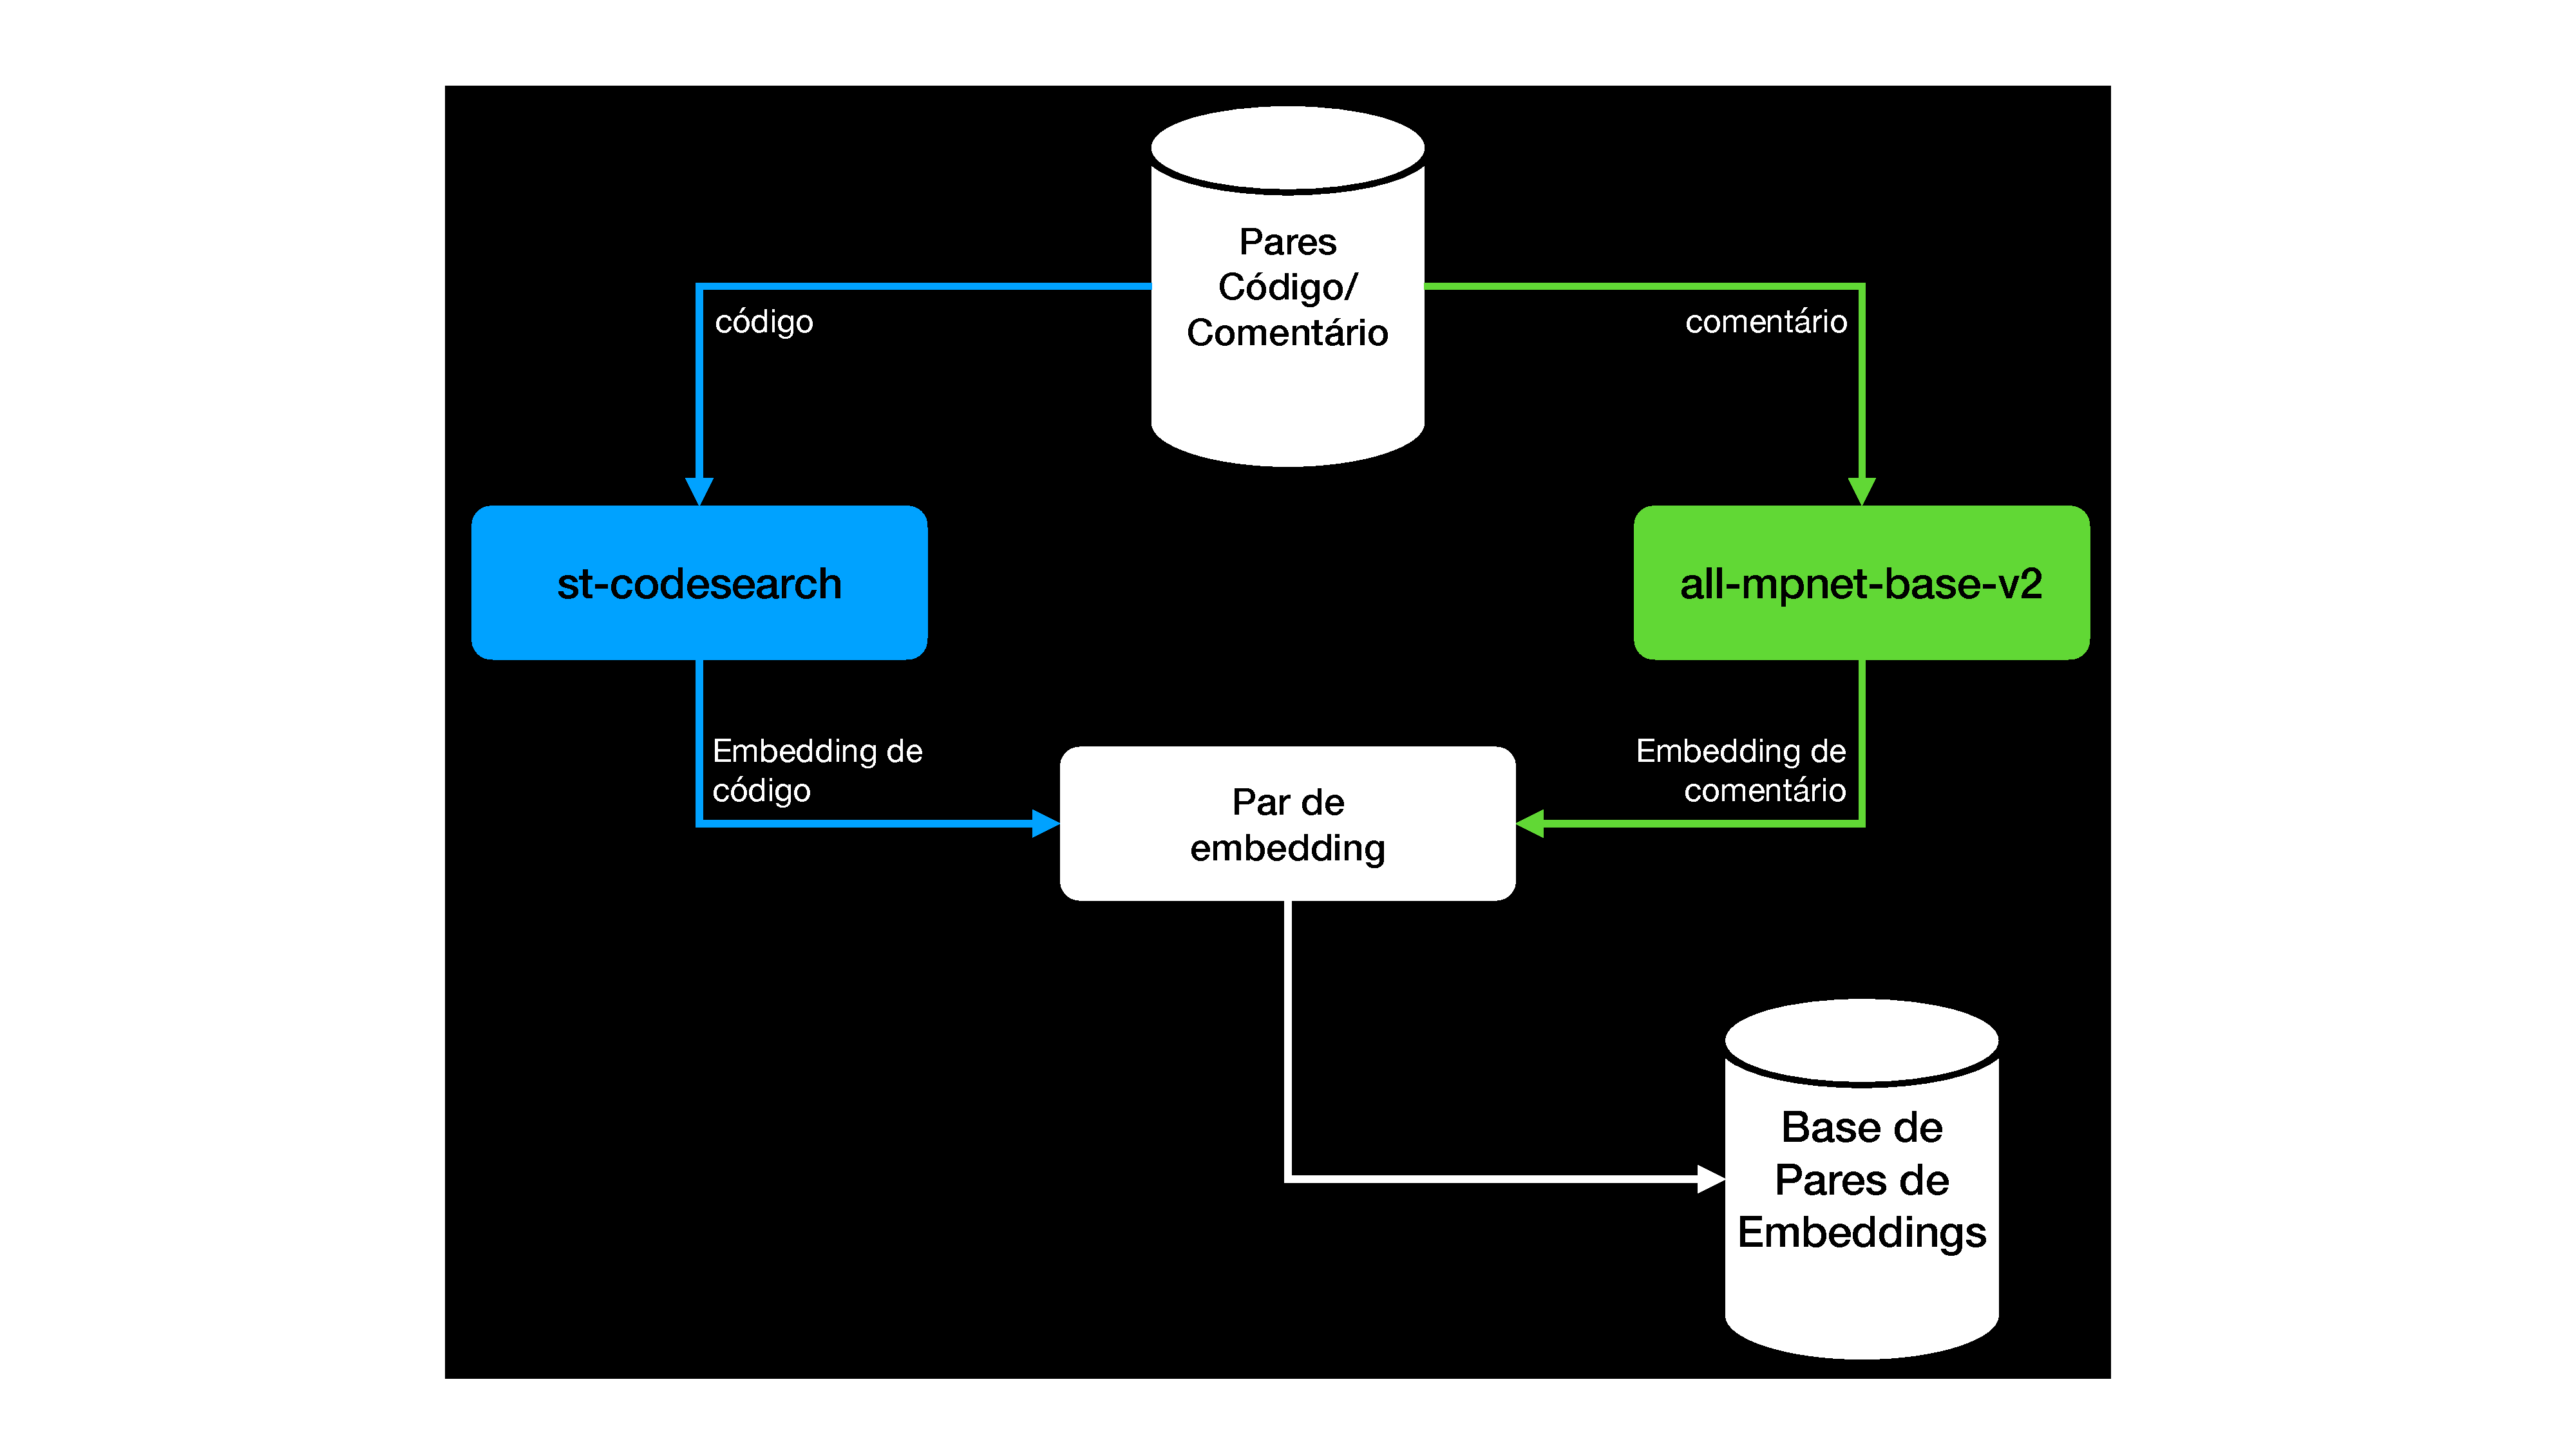
\includegraphics[scale=0.35]{db_embeddings.pdf}
        \smallcaption{Fonte: Autor}
        \label{fig:metodology-db-embeddings}
\end{figure}

\section{Modelo de comparação de \textit{embeddings}}
\label{sec:methodology:embedding-comparator}

O modelo de comparação consiste em uma rede neural \gls{mlp}, que tem como entrada dois \textit{embeddings}: um \textit{embedding} de código-fonte e outro do comentário, e como saída um valor racional dentro do intervalo [0, 1]. Este valor de saída determinará a similaridade entre os \textit{embeddings} de código-fonte e comentário.

Inicialmente, o modelo realiza a concatenação dos dois \textit{embeddings} de entrada. Essa concatenação é feita juntando os dois vetores em um só, de forma que dado um \textit{embedding} de código-fonte de tamanho $m$, e um \textit{embedding} de comentário de tamanho $n$, o tamanho do vetor resultante após a concatenação será $m + n$. No presente estudo, os modelos transformers utilizados geram \textit{embeddings} de tamanho 768 - portanto, o tamanho do vetor concatenado foi de 1536.

Além disso, tal modelo de comparação possui com 4 camadas densas intermediárias com 200, 150, 100 e 50 neurônios, respectivamente, enquanto a camada de saída possui apenas um neurônio. Duas funções de ativação foram utilizadas neste modelo: uma para as camadas intermediárias e outra para a camada de saída. As camadas intermediárias utilizam a função de ativação \gls{relu}, enquanto a camada de saída utiliza a função de ativação sigmoide.

\section{Etapa de treinamento}
\label{sec:methodology:embedding-comparator-training}
Durante o treinamento do modelo de comparação, foram utilizados 2000 pares de código-fonte/comentário, todos da linguagem \textit{Python}. Como a base de pares utilizada não possui exemplos negativos, estes foram gerados durante a etapa de treinamento.

Um exemplo negativo consiste em um par código-fonte/comentário onde o comentário não descreve o código-fonte correspondente. Com isso, para cada par código-fonte/comentário, foi gerado $neg\_samples\_per\_sample$ pares negativos para o treinamento do modelo de comparacão. Para este parâmetro, foram utilizados os valores 1, 5 e 15. Como a base de treinamento possui tamanho 2000, o tamanho final da base de treinamento após a geração dos pares negativos foi de 4000, 12000 e 32000 pares, respectivamente.

Tais pares negativos foram gerados da seguinte forma: o modelo em questão foi treinado com o \textit{batch\_size} de 200. Com isso, para cada par contido no \textit{batch}, são escolhidos $neg\_samples\_per\_sample$ pares de forma aleatória dentro do \textit{batch} atual, excluindo o par em questão para que não haja falsos pares negativos. Por fim, dado que o par positivo consiste em um código-fonte $cod\_p$ e um comentário $com\_p$, e que um par negativo contenha um código-fonte $cod\_n$ e um comentário $com\_n$, é então gerado, para cada par negativo escolhido, um par código-fonte/comentário da forma $(cod\_p, com\_n)$. A Figura \ref{fig:metodology-neg_samples_gen_diagram} ilustra esse processo de geração de pares negativos.

\begin{figure}[H]
    \centering
        \caption{Geração de pares código-fonte/comentário negativos}
        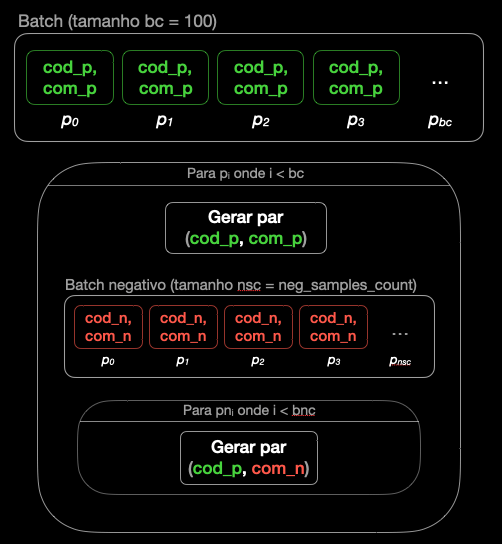
\includegraphics[scale=0.7]{neg_samples_gen.png}
        \smallcaption{Fonte: Autor}
        \label{fig:metodology-neg_samples_gen_diagram}
\end{figure}

\section{Busca de código-fonte}
Essa etapa é responsável por buscar trechos de código-fonte dado uma \textit{query} escrita em na língua inglesa, haja vista que os pares código/comentário utilizados para treinamento só possuem comentários em inglês.

Como é possível ver na Figura \ref{fig:metodology-system_overview}, inicialmente o sistema gera o \textit{embedding} para a \textit{query} dada, utilizando o modelo \textit{transformer} de linguagem natural selecionado neste estudo. Depois, para cada par código-fonte/comentário da base de treino, é obtido o embedding de código desse par, o qual, junto com o \textit{embedding} da query, serve de entrada para o modelo de comparação. A similaridade resultante é então adicionada ao ranking de similaridade, que por sua vez, consiste em uma lista de trechos de código-fonte, ordenada de forma decrescente pelo valor de similaridade.

\section{Materiais}
Tanto o treinamento da rede quanto os experimentos descritos no capítulo \ref{chp:experiments} foram realizados utilizando um computador modelo Macbook Pro, com processador Apple M2 Pro com 10 núcleos, 32 GB de memória RAM e 1TB de capacidade de armazenamento.
\chapter{PROPOSTA EXPERIMENTAL}
\label{chp:experiments}

Para o estudo em questão, propõe-se três experimentos que avaliarão tanto a capacidade de generalização do modelo de comparação de \textit{embeddings} quanto sua eficácia no problema de busca de código-fonte a partir de linguagem natural. As descrições e objetivos de cada experimento estão nas seções seguintes deste capítulo.

\section{Experimento 1}
\label{sec:experiments:experiment-1}
O objetivo desse experimento é determinar a capacidade de generalização do modelo de comparação.

Para tanto, foram utilizados os 100 primeiros pares código-fonte/comentário da base de treinamento. Para cada par p, removeu-se uma palavra aleatória do comentário, gerando uma \textit{query} $C^-$, a qual foi gerado um \textit{embedding} utilizando o modelo \textit{all-mpnet-base-v2} - mesmo modelo de linguagem natural utilizado na geração da base de \textit{embeddings}. Depois, o \textit{embedding} de código-fonte é recuperado da base de pares \textit{embeddings}. 

Com isso, tem-se o \textit{embedding} de $C^-$ $Emb_{c-}$, e o \textit{embedding} de código-fonte $Emb_{cod}$, os quais serviram de entrada para o modelo de comparação. Este processo foi repetido $c\_count$ vezes, onde $c\_count$ é dado por $c\_count = min(n_{pc}, 30)$ e $n_{pc}$ o qual $n_{pc}$ corresponde ao número de palavras do comentário. As palavras foram removidas de forma aleatória, e foi determinado o máximo de 30 interações caso o comentário do par em questão seja muito grande. A Figura \ref{fig:experiment-1-diagram} ilustra o experimento em questão.

\begin{figure}[H]
    \centering
        \caption{Diagrama do experimento 1}
        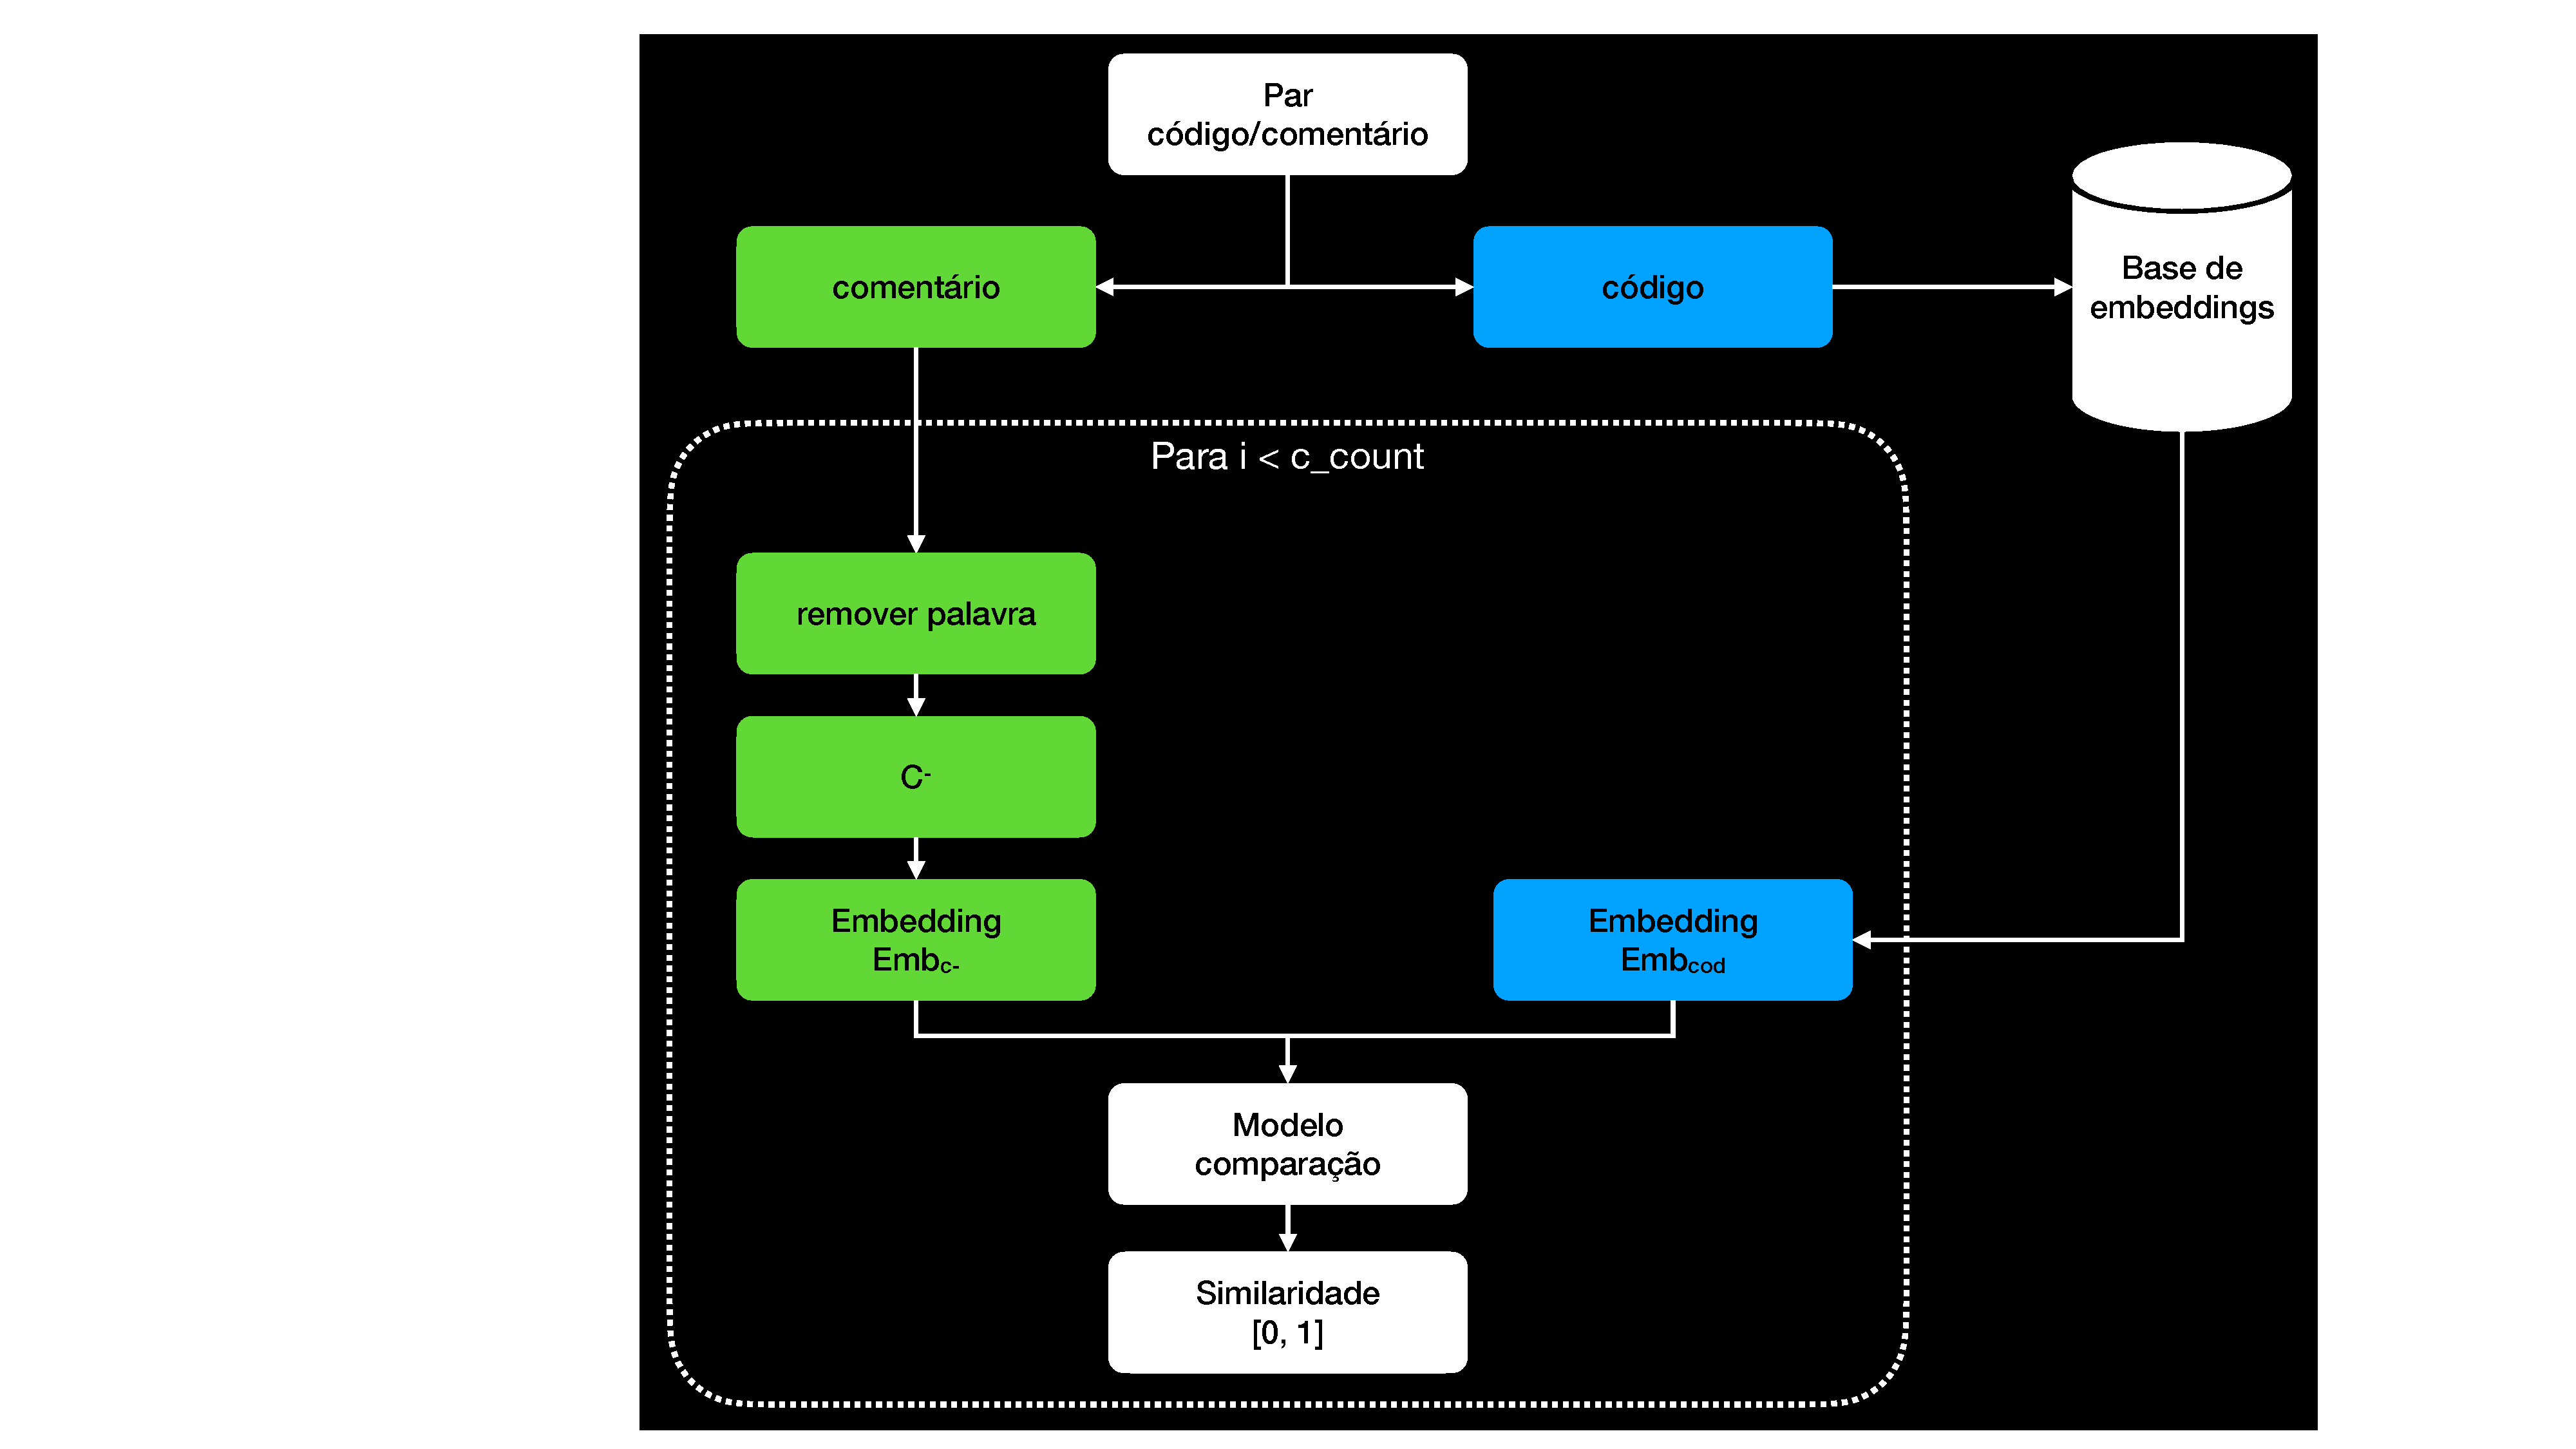
\includegraphics[scale=0.3]{imagens/proposta-experimental/experiment-1.pdf}
        \smallcaption{Fonte: Autor.}
        \label{fig:experiment-1-diagram}
\end{figure}

Para este experimento, espera-se que, ao remover uma palavra semanticamente importante para o par código/comentário, a similaridade seja baixa. De igual modo, quando uma palavra menos importante for removida, espera-se que a similaridade seja alta.

\section{Experimento 2}
\label{sec:experiments:experiment-2}
O objetivo desse experimento é avaliar a performance do modelo de comparação no problema de busca de código-fonte a partir de linguagem natural.

Neste experimento, utilizou-se todos os pares da base de treinamento. Para cada par, foi feito uma busca utilizando seu comentário como \textit{query}. Portanto, a posição do resultado mais importante - o $rank_i$ - será a posição que este par aparecerá no ranking de similaridade. Como a base de treino possui 2000 pares, serão realizadas 2000 buscas e as métricas \gls{mrr} e \textit{SuccessRate@k} com com $k=1$, $k=5$ e $k=10$ para avaliação da performance do modelo de comparação.

A busca de código-fonte no presente trabalho é feita da seguinte forma: dado uma \textit{query} $Q$, é gerado um \textit{embedding} $Emb_q$ a partir da \textit{query} $Q$. Depois, para cada \textit{embedding} de código-fonte $Emb_{cod}$ presente na base de \textit{embeddings}, utiliza-se o modelo de comparação para determinar a similaridade entre $Emb_q$ e $Emb_{cod}$, gerando uma ranking de resultados, ordenado pela similaridade de forma decrescente. A Figura \ref{fig:metodology-system_overview} ilustra o processo de busca descrito, bem como a Figura \ref{fig:experiment-2-diagram} apresenta o diagrama do experimento em questão.

\begin{figure}[H]
    \centering
        \caption{Diagrama do experimento 2}
        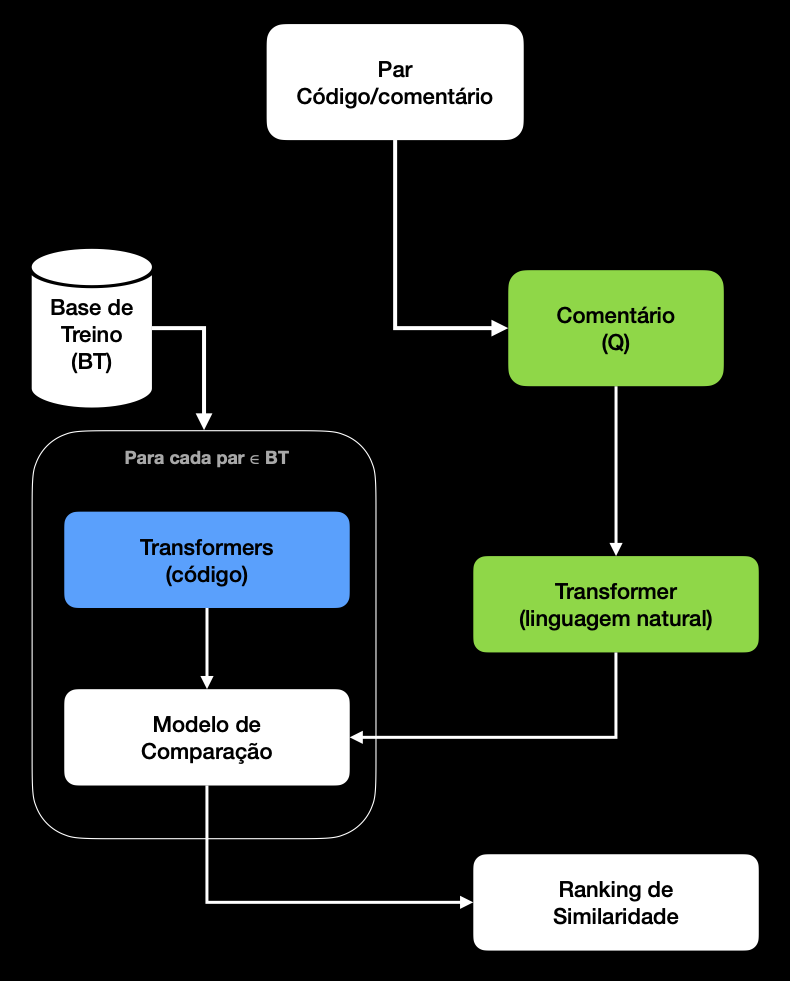
\includegraphics[scale=0.5]{imagens/proposta-experimental/experiment-2.png}
        \smallcaption{Fonte: Autor.}
        \label{fig:experiment-2-diagram}
\end{figure}

\section{Experimento 3}
\label{sec:experiments:experiment-3}
O objetivo desse experimento é determinar a acurácia do modelo de comparação, utilizando as \textit{queries} disponíveis na base de dados \textit{CodeSearchNet}. Ao todo, a base em questão contém 4009 amostras, cada uma contendo os seguintes dados:

\begin{itemize}
    \item \textit{Query}: Termo, em linguagem natural, utilizado para busca de código-fonte
    \item \textit{Language}: Linguagem de programação do código-fonte associado
    \item \textit{GitHubUrl}: Link do Github para o código-fonte associado
    \item \textit{Relevance}: Valor inteiro, entre 0 e 3 (inclusivo), que representa o quão a \textit{Query} é relevante ao código-fonte em questão. 0 signfica que o código-fonte é pouco relevante para a query, e 3 signfica que o código é altamente relevante para a \textit{Query}.
    \item \textit{Notes}: Anotações, em linguagem natural, feitas pelos criadores dessa base de dados, caso julgassem relevante para a amostra em questão.
\end{itemize}

Para o experimento em questão, foram utilizadas apenas as amostras da linguagem \textit{Python}. Além disso, amostras duplicadas e aquelas cujo o campo \textit{GitHubUrl} não foi encontrado na base \textit{CodeSearchNet} também foram filtradas. Por fim, 842 amostras de \textit{queries} foram utilizadas neste experimento. 

Com isso, para cada uma das 842 amostras disponíveis, foi gerado o \textit{embedding} para o campo \textit{Query} utilizando o \textit{transformer} de linguagem natural. Na parte do código, utilizou-se o campo \textit{GitHubUrl} para buscar o código correspondente na base \textit{CodeSearchNet}, e foi gerado o \textit{embedding} para esse código utilizando o \textit{transformer} de código-fonte. Ambos os modelos \textit{transformers} citados (de linguagem natural e de código-fonte) são os mesmos utilizados nos experimentos anteriores. O modelo de comparação foi então utilizado para determinar a similaridade entre esses dois \textit{embeddings}, conforme mostrado na Figura \ref{fig:experiment-3-diagram}. Vale ressaltar que o presente expeirmento não realiza o processo de busca de código-fonte - antes, este visa comparar a saída do modelo de comparação com o padrão estabelecido pelo repositório \textit{CodeSearchNet}, através do campo \textit{Relevance}. Por isso, as métricas \gls{mrr} e \textit{SuccessRate@k} não foram aplicadas no presente experimento.

Como o modelo de comparação proposto neste estudo gera resultados no intervalo $[0, 1]$, e o campo \textit{Relevance} possui valores inteiros entre 0 e 3, foi necessário uma normalização para determinar se o modelo categorizou o par $(Emb_{qcs}, Emb_{cod})$ de acordo com a relevância esperada. Para tanto, dividiu-se os dois intervalos ao meio, ou seja, para valores de \textit{Relevance} 0 ou 1, espera-se que a similaridade seja igual ou menor à 0.5, bem como para \textit{Relevance} 2 ou 3, espera-se similaridades maiores que 0.5. Como exemplo, caso a similaridade dada pelo modelo de comparacão for de $0.4$, e a relevância esperada para esta amostra seja 0, considera-se um acerto do modelo de comparação. Ainda, se a similaridade for $0.6$ e a relevância 1, considera-se um erro do modelo.

\begin{figure}[H]
    \centering
        \caption{Diagrama do experimento 3}
        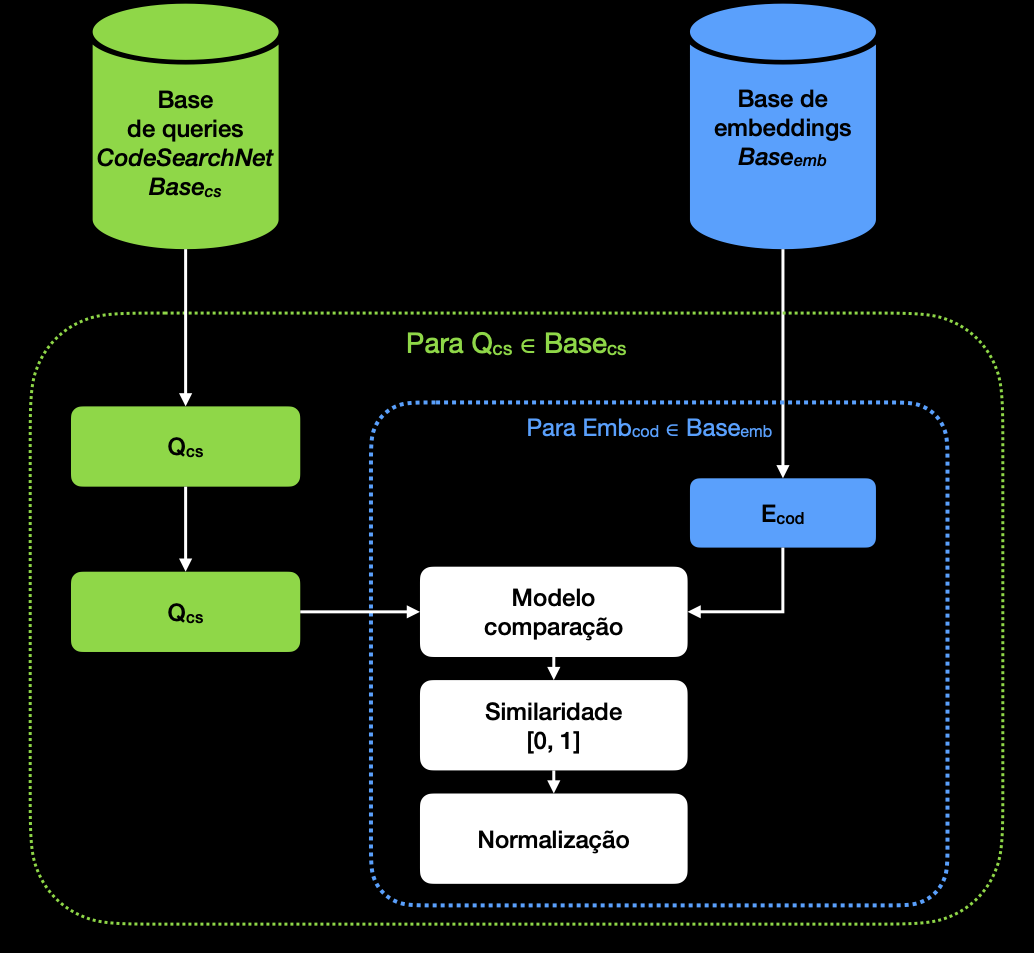
\includegraphics[scale=0.4]{imagens/proposta-experimental/experiment-3.png}
        \smallcaption{Fonte: Autor}
        \label{fig:experiment-3-diagram}
\end{figure}

\chapter{RESULTADOS}
\label{chp:results}

Este capítulo apresenta os resultados dos três experimentos descritos no capítulo \ref{chp:experiments}. Os resultados serão divididos em três seções, uma para cada experimento.

\section{Experimento 1} 
\label{sec:results:experiment-1}

Conforme descrito no capítulo \ref{chp:experiments}, este experimento utiliza 100 pares código-fonte/comentário da base de treinamento para determinar a capacidade semântica do modelo de comparação, através da remoção de palavras aleatórias do comentário.

A Figura \ref{fig:experiment-1:good} apresenta um resultado positivo de um dos 100 pares utilizados.
\begin{figure}[H]
  \centering
    \caption{Exemplo de resultado positivo}
    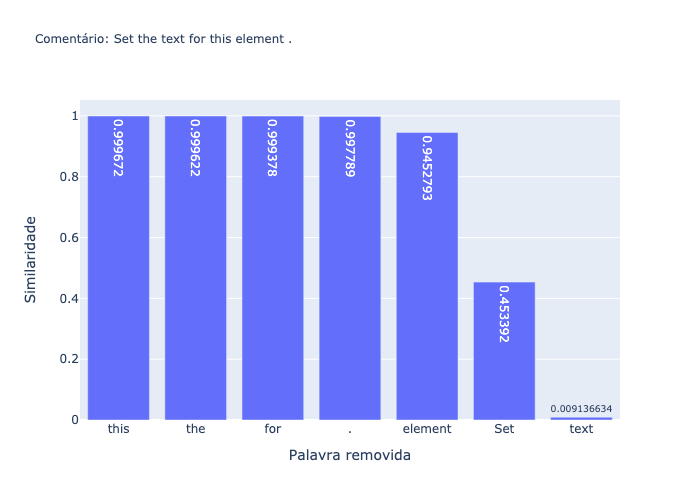
\includegraphics[scale=0.6]{imagens/resultados/experiment-1/sample_5.png}
    \smallcaption{Fonte: Autor}
    \label{fig:experiment-1:good}
\end{figure}

Na Figura \ref{fig:experiment-1:good}, gráfico mostra o comentário do par selecionado, a palavra removida (eixo x) e a similaridade (eixo y) obtida pelo modelo de comparação. Vale lembrar que ao remover uma palavra do comentário, obtem-se a \textit{query} $C^-$. Isso significa que, usando os dados da Figura \ref{fig:experiment-1:good} como exemplo, dado que o comentário é \textit{Set the text for this element.}, ao remover a palavra \textit{this}, obteve-se a \textit{query} $C^-$ \textit{Set the text for element.}.

Vale lembrar que o modelo de comparação foi treinado utilizando como entrada os \textit{embeddings} de código-fonte e do seu respectivo comentário. Portanto, valores de similaridade altos neste experimento indicam que o modelo não considerou a palavra removida importante para a busca; de igual modo, similaridade baixa indica que a palavra removida era importante para o par em questão.

O resultado da Figura \ref{fig:experiment-1:good} é considerado positivo pois, ao se retirar palavras menos relevantes do comentário, a similaridade se manteve alta - como se tivéssemos utilizado o próprio comentário como \textit{query}. De igual modo, quando palavras relevantes foram removidas, a similaridade diminuiu como pode-se notar nas similaridades das palavras \textit{text} e \textit{Set}.

Outro ponto interessante desse resultado é notar que o modelo conseguiu captar informações semânticas do comentário. A Figura \ref{fig:experiment-1-medium} mostra o par código-fonte/comentário em questão.

\begin{figure}[H]
  \centering
    \caption{Exemplo de resultado positivo}
    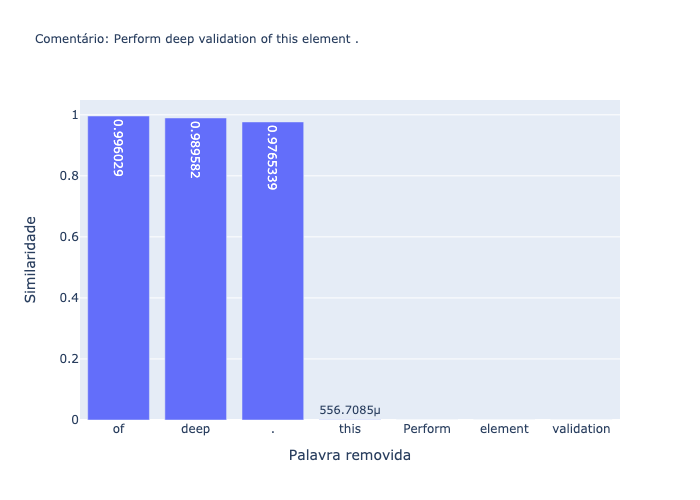
\includegraphics[scale=0.6]{imagens/resultados/experiment-1/sample_9.png}
    \smallcaption{Fonte: Autor}
  \label{fig:experiment-1-medium}
\end{figure}

A Figura \ref{fig:experiment-1-medium} mostra que o trecho de código-fonte em questão é responsável por atribuir (\textit{set}) dada palavra, chamada pelo autor do código de \textit{text}, ao valor de \textit{TextContent}. Com isso, as palavras \textit{text}, \textit{set} e \textit{content} são semanticamente importantes nesse par, o que corrobora os resultados apresentados na Figura \ref{fig:experiment-1:good}.

Em outro par, o modelo acertou a maioria das palavras relevantes, conforme apresentado na Figura \ref{fig:experiment-1-medium}.

Os resultados do modelo mostram que, para o comentário \textit{Perform deep validation of this element.}, as palavras \textit{validation}, \textit{element} e \textit{Perform} são semanticamente relevante para o par em questão, o que é verdade. Entretanto, o modelo também considerou relevante a palavra \textit{this}, e não considerou importante a palavra \textit{deep} o que, dado o contexto, seria exatamente ao contrário: \textit{this} deveria ser significativamente menos relevante do que \textit{deep}.

Por fim, a Figura \ref{fig:experiment-1-bad} apresenta um par onde o modelo não conseguiu detectar o significado semântico das palavras do comentário.

\begin{figure}[H]
  \centering
    \caption{Exemplo de resultado negativo}
    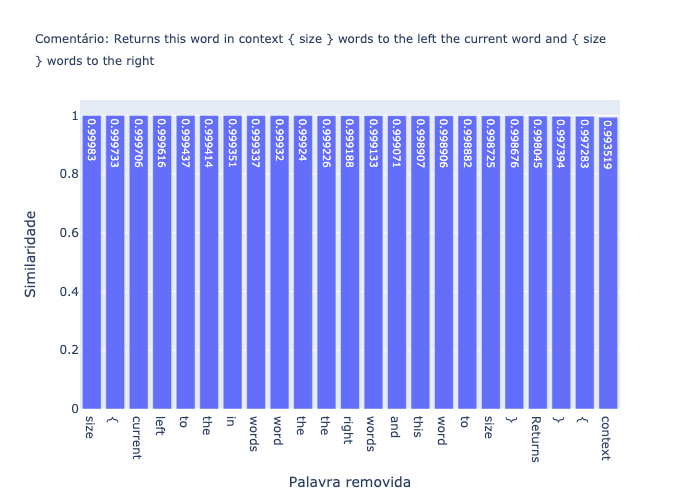
\includegraphics[scale=0.6]{imagens/resultados/experiment-1/sample_29.png}
    \smallcaption{Fonte: Autor}
    \label{fig:experiment-1-bad}
\end{figure}

Na Figura \ref{fig:experiment-1-bad} é possível ver que todas as palavras retiradas obtiveram valores muito próximos de similaridade, o que representa que o modelo de comparação não conseguiu determinar quais palavras eram semanticamente relevantes para o par em questão. Além disso, verificou-se nesse experimento que, quando o par possui comentário com 20 palavras ou mais, esses resultados geralmente se repetem, ou seja, o modelo não consegue determinar quais palavras são mais relevantes para o par em questão. Uma possível explicação seja que, dado o tamanho do comentário e do código-fonte, o modelo não consiga extrair informações sobre o contexto do par e, portanto, não consegue determinar as palavras mais relevantes.

Por fim, 100 pares código-fonte/comentário foram utilizados durante este experimento, gerando 1439 $C^-$, com tempo de execução de 1 minuto e 40 segundos.

\section{Experimento 2} 
\label{sec:results:experiment-2}
O objetivo desse experimento é determinar a performance do modelo de comparação na tarefa de busca de código-fonte a partir de linguagem natural. Para tanto, utilizou-se as mesmas 100 pares código-fonte/comentário do experimento 1, além das métricas de recuperação de informação \gls{mrr} e \textit{SuccessRate@k} com $k=1$, $k=5$ e $k=10$. Foi aplicado o mesmo processo de geração de \textit{queries} $C^-$ utilizado no experimento 1. Portanto, para cada par, realizou-se uma busca de código-fonte para cada uma das \textit{queries} $C^-$ geradas. 

Aqui, da lista de resultados resultante de cada busca, considera-se que o código-fonte do par em questão é o mais relevante. Portanto, ao se fazer uma busca utilizando a \textit{query} $C^-$ gerada a partir do comentário do $par_i$, o código-fonte mais relevante da lista de resultados será o código-fonte do mesmo $par_i$. Inclusive, a posição desse código-fonte na lista de resultados será utilizada para calcular as métricas \gls{mrr} e \textit{SuccessRate@k}.

Portanto, a Figura \ref{fig:experiment-2-mrr} mostra os valores de \gls{mrr} para cada um dos 100 pares utilizados. Neste experimento, o menor valor de \gls{mrr} foi de $0.008$ enquanto o maior foi de $0.783$. Ainda, a média de todos os valores obtidos de \gls{mrr} foi de aproximadamente $0.130$.

\begin{figure}[H]
  \centering
      \caption{\textit{MRR}}
      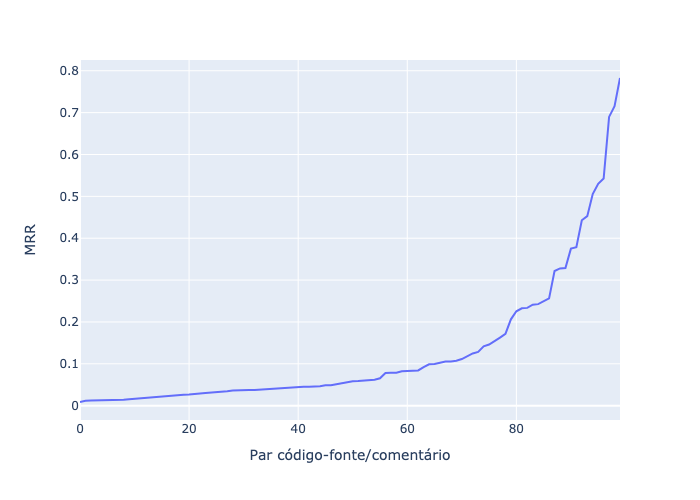
\includegraphics[scale=0.6]{imagens/resultados/experiment-2/mrr.png}
      \smallcaption{Fonte: Autor}
      \label{fig:experiment-2-mrr}
\end{figure}


Em relação ao \textit{SuccessRate@k}, a Figura \ref{fig:experiment-2-success-k} mostra os resultados obtidos para $k=1$, $k=5$ e $k=10$. Com esses valores de $k$, os maiores resultados obtidos foram de $0.933$, $0.960$ e $1.000$, respectivamente, enquanto o menor resultado foi zero para todos os valores de $k$. A média dos resultados foi de, aproximadamente, $0.044$, $0.176$, $0.297$ para os valores de $k=1$, $k=5$ e $k=10$, respectivamente.

\begin{figure}[H]
  \centering
      \caption{\textit{SuccessRate@k}}
      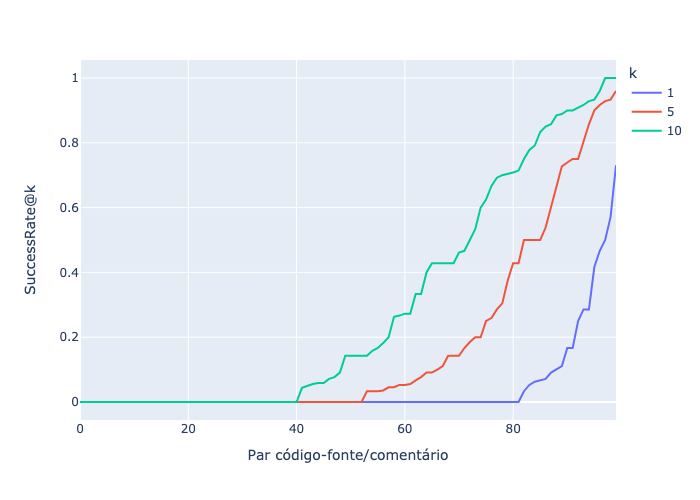
\includegraphics[scale=0.6]{imagens/resultados/experiment-2/success-rates.png}
      \smallcaption{Fonte: Autor}
      \label{fig:experiment-2-success-k}
\end{figure}

Por fim, o tempo total de execução desse experimento foi de 27 minutos e 55 segundos.

\section{Experimento 3} 
\label{sec:results:experiment-3}
Por fim, o experimento 3 utiliza as \textit{queries} $Q_{cs}$ da base de dados \textit{CodeSearchNet}, bem como os valores esperados para cada \textit{query} $Q_{cs}$, também contidos na base \textit{CodeSearchNet}, para determinar a quantidade de acertos do modelo de comparação utilizando os dados contidos na base em questão. O objetivo é determinar a performance do modelo de comparação proposto neste estudo com o padrão estabelecido pelos autores da base \textit{CodeSearchNet}. Este valor é chamado pelos autores de relevância.

Para determinar se o modelo obteve o valor correto em relação ao esperado para determinada \textit{query}, foi realizado uma normalização do valor de similaridade em relação ao valor esperado. Com isso, espera-se que valores de similaridade iguais ou menores que $0.5$ possuam relevância de 0 ou 1, enquanto valores de similaridade maiores que $0.5$ tenham relevância igual a 2 ou 3, conforme descrito na seção \ref{sec:experiments:experiment-3}.

Portanto, utilizando os parâmetros contidos na base de dados \textit{CodeSearchNet} \cite{Husain2019CodeSearchNetCE}, o modelo de comparação obteve $54.99\%$ de acerto, com 463 predições corretas de 842 \textit{queries}. Além disso, o tempo de execução do experimento em questão foi de $13.6$ segundos.


\chapter{Discussões}
\label{chp:discussions}

A seguir serão apresentadas discussões sobre os resultados apresentados no capítulo \ref{chp:results}, bem como limitações do sistema proposto neste estudo, e trabalhos futuros na área de busca de código-fonte por linguagem natural. Por fim, serão relacionadas as contribuições do presente estudo.

No experimento 1, houveram amostras onde todas as palavras retiradas geraram praticamente o mesmo valor de acurácia, ou ainda amostras onde a redução de acurácia aconteceu em stop-words ou outras palavras não tão relevantes para aquele comentário em questão. Com isso, tendo em mente que a entrada do modelo de comparação são dois \textit{embeddings} com tamanho 768, e gerados por redes \textit{transformers} complexas, é possível que o modelo de comparação, o qual é propositalmente mais simples que os geradores de \textit{embeddings} utilizados, não tenha conseguido generalizar todas informações semânticas contidas nos embeddings de entrada.

Entretando, os resultados do experimento 1 também mostraram que, para parte das amostras, a retirada de palavras importantes do comentário reduziu notavelmente a similaridade obtida, o que indica que a rede conseguiu captar o significado semântico destas palavras retiradas no comentário original. Algumas amostras, porém, obtiveram diferenças de acurácia menores do que outras. Essa diferença menor de acurácia entre amostras também pode ser explicada, já que apesar de uma palavra importante estar sendo removida do comentário, o \textit{embedding} de código-fonte será idêntico para todas as queries $C^-$ geradas para essa amostra, o que significa que ao menos 50\% da entrada do modelo de comparação será igual. Portanto, diferenças substanciais da similaridade, apenas removendo uma palavra do comentário original, mostra o potencial do modelo de comparação proposto neste estudo.

No experimento 2, os valores obtidos nas métricas \gls{mrr} e \textit{SuccessRate@k} foram baixos quando comparados diretamente com outros estudos presentes na literatura, conforme mostrado na Figura \ref{fig:results:experiment-2}. \textcite{Gu2018DeepCS}, por exemplo, obteve $0.367$ e $0.465$ nas métricas \textit{SuccessRate@1} e \gls{mrr}, respectivamente, enquanto \textcite{Gu2021CRaDLeDC} obteve $0.791$ e $0.843$ nas mesmas métricas, respectivamente. Entretanto, não é possível comparar diretamente tais resultados, já que os experimentos feitos no presente estudo diferem dos experimentos realizados pelos trabalhos citados. No presente estudo, foram utilizados apenas pares da linguagem \textit{Python}, e destes pares, 2000 amostras foram utilizadas tanto no treino quanto nesse experimento.

Por outro lado, obteve-se bons tempos de execução tanto para o treinamento quanto para a conclusão do experimento 2, sendo estes tempos de 48 minutos e 39 minutos e 45 segundos, respectivamente. Vale ressaltar que o modelo foi treinado sem \textit{hardware} dedicado (como placa de vídeo, por exemplo), e durante o desenvolvimento do presente estudo, bibliotecas como \textit{Keras} e \textit{TensorFlow} não estavam totalmente otimizadas para trabalhar com o processador \textit{Apple} M2 Pro, utilizado para desenvolvimento desse trabalho.

Por fim, o experimento 3 foi feito utilizando queries e valores de relevância disponíveis na base de dados \textit{CodeSearchNet}, conforme descrito na seção \ref{sec:experiments:experiment-3}. Aqui, utilizou-se tanto as queries disponíveis na base em questão, como suas respectivas relevâncias em relação a determinado trecho de código-fonte, disponíveis na mesma base. Além disso, muitos trechos de código-fonte dessa base de queries não foram utilizados nos experimentos 1 e 2. Por conta desses fatores, não foi possível utilizar métricas de recuperação de informação como \gls{mrr} ou \textit{SuccessRate@k}. Com isso, para este experimento, foi utilizado a similaridade (resultante do modelo de comparação) e o valor de relevância para determinar se o resultado do modelo de comparação está correto ou não.

\section{Limitações e trabalhos futuros}
\label{sec:discussions:future-works}

Durante o desenvolvimento deste trabalho, foram encontradas limitações em relação ao sistema proposto. Uma das limitações foi o tamanho dos \textit{embeddings} gerados, tanto para comentário quanto para código-fonte. Os modelos de \textit{embeddings} utilizados no presente estudo geram \textit{embeddings} de tamanho fixo, a saber, 768: caso o tamanho da entrada desses modelos seja maior do que 768, o vetor resultante será truncado; caso contrário, será adicionado um valor neutro de \textit{padding} no final do \textit{embedding} para atingir o tamanho desejado. Portanto, apesar de quaisquer modelos de embedding poderem ser usados no sistema proposto, o modelo de comparação espera \textit{embeddings} de tamanho 768, tanto para comentário quanto para código-fonte.

Outra limitação é a topologia utilizada no modelo de comparação. Propositalmente, o modelo de comparação utilizou uma rede \gls{mlp}, a qual é mais simples tanto em relação à outras redes neurais (como \gls{lstm}, por exemplo), quanto em relação aos modelos de \textit{embedding} utilizados neste trabalho, os quais são baseados em redes \textit{transformers}. Foram dois motivos que levaram a utilização de uma topologia mais simples para o modelo de comparação: o primeiro foi os requisitos computacionais. Redes \gls{mlp}, por serem mais simples, requerem muito menos recursos computacionais para treinamento do que uma rede baseada em \textit{transformer}, por exemplo. O segundo motivo foi justamente analisar como uma topologia mais simples se comportaria com entradas geradas por modelos mais complexos.

Diante disso, uma recomendação para trabalhos futuros seria utilizar outras topologias para comparação de embeddings. Antes dos modelos \textit{transformers} serem o estado da arte na área de \gls{nlp}, esse posto era ocupado pelas redes recorrentes como \gls{lstm}, por exemplo. Portanto, seria interessante validar se tais redes, apesar de mais complexas e, portanto, demandarem mais recursos computacionais que o modelo de comparação proposto no presente estudo, podem generalizar melhor as informações contidas nos \textit{embeddings} e, com isso, gerarem melhores resultados na busca de código-fonte a partir de linguagem natural.

Além disso, no presente estudo utilizou-se apenas uma combinação de modelos de embeddings para comentário e código-fonte. Em trabalhos futuros, pode-se utilizar outros modelos de embedding, tanto para linguagem natural (comentário) quanto para código-fonte. Inclusive, tais modelos de embedding não precisam, necessariamente, serem baseados em transformers, embora hoje esses sejam o estado da arte. Modelos de embedding como \gls{nbow}, por exemplo, também podem ser utilizados no sistema em questão.

Ainda, cita-se também a possibilidade de, em trabalhos futuros, de ajustar os parâmetros da rede \gls{mlp} utilizada para o atual modelo de comparação, a fim de melhorar a performance do sistema. Parâmetros como número e tipo de camadas intermediárias, tamanho dos embeddings de entrada e funções de ativação (tanto das camadas intermediárias quanto da camada de saída), podem facilmente ser alterados a fim de aperfeiçoar o sistema proposto. Além disso, os resultados do experimento 1 apontam que quanto maior o tamanaho do comentário, menor a eficácia da rede em determinar palavras semanticamente relevantes, embora essa regra não se aplique a todas as amostras utilizadas. Com isso, a remoção de palavras não relevantes (\textit{stop words}) durante o treinamento do modelo de comparação pode também melhorar sua performance.

Outra possibilidade para trabalhos futuros seria utilizar redes mais complexas para o modelo de comparação. Como redes recorrentes eram o estado da arte antes do advento dos modelos \textit{transformers}, substituir a atual rede \gls{mlp} por uma outra topologia como \gls{lstm} pode melhorar os resultados obtidos no presente estudo.

Por fim, os resultados obtidos na presente pesquisa foram submetidos à revista Journal of Systems and Software.
\chapter{CONCLUSÃO}
\label{chp:conclusao}

A busca de código-fonte a partir de linguagem natural é uma tarefa essencial para engenheiros de \textit{software} nas mais diversas áreas da indústria \cite{Sadowski2015HowDS}. Como visto no capítulo \ref{chp:relatedWorks}, inúmeros trabalhos relacionados à busca de código-fonte tem sido publicados nos últimos anos. 

Atualmente, os modelos \textit{transformers} são os mais utilizados no problema de busca de código-fonte, devido, principalmente, à sua capacidade de extrair informações semânticas dos dados de entrada, como \textit{queries} em linguagem natural para busca de código-fonte. Diversos modelos \textit{transformers} pré treinados estão disponíveis atualmente. Porém, para adaptar tais modelos para dado problema específico, estes demandam consideráveis quantidades de recursos computacionais, tanto para serem treinados novamente quanto para o \textit{fine tuning}. 

Diante disso, o presente trabalho implementou um sistema de busca de código-fonte a partir de linguagem natural, utilizando uma rede \gls{mlp} para determinar a similaridade entre dois \textit{embeddings}, gerados por dois modelos \textit{transformers} pré treinados: um em linguagem natural, e outro em linguagem de programação. O modelo de comparacão, o qual consiste em uma rede \gls{mlp}, foi treinado com pares de \textit{embeddings} código-fonte/comentário, a fim de determinar o grau de similaridade entre um texto escrito em linguagem natural (\textit{query}) e um trecho de código-fonte.

Implementou-se três experimentos para avaliar a performance do sistema proposto. Dos resultados, analisando 100 pares código-fonte/comentário da base de treinamento, obteve-se $0.130$ de média de \gls{mrr}, além das médias $0.044$, $0.176$, $0.297$ para os valores de $k=1$, $k=5$ e $k=10$ da métrica \textit{SuccessRate@k}. Embora o modelo não tenha obtido uma média de resultados expressiva, dois pontos são importantes de serem mencionados. O primeiro é que não é possível realizar uma comparação direta desses valores obtidos no presente estudo com resultados de trabalhos como \textcite{Gu2018DeepCS} ou \textcite{Gu2021CRaDLeDC}, já que os experimentos conduzidos nestes trabalhos foram diferentes dos realizados no presente trabalho. Segundo, que apesar da média obtida ter sido baixa, o modelo obteve bons resultados para alguns pares testados, tanto no experimento de generalização quanto nos de busca, o que indica que trabalhos futuros podem ser realizados a partir deste, a fim de melhorar a performance geral do modelo de comparação.


\printbibliography

% \printindex

\end{document}
